\chapter{Laboratory Testing - Results and Discussion}
\label{chap:results}
\todo[inline, color = red!60]{burde signaturplottene komme først? og så analysen basert på disse?}

In this chapter, the results from the laboratory testing is presented. The first results are plots from the principal component analysis, first conducted with microplastic alone, before running an additional analysis, adding biological components to the test set. The second results are plots presenting the specific signatures of the tested microplastic. In this chapter, the results will be presented, compared and discussed along the way. 

%Merk at vi egentlig mener at diskusjonen i seg selv er en del av resultatet! Bruk diskursjon som et underpunkt til resultat

\begin{comment}
\section{Results from the Spectrometer I} 
the wave spectrum from one of the types. This can be compared to the associated colors wave spectrum. 
\section{Results from the Spectrometer II}
Comparing the signature of two different types of plastic (de gjennomsiktige pelletsene), which more or less have the same signature
\section{Principal Component Analysis I}
Using the different types of plastic only

\section{Principal Component Analysis II} 
The plastic types compared with algae

\section{The Final Method} 
\end{comment}

\section{Principal Component Analysis}

As mentioned in the previous sections, the results from scanning the plastic samples using hyper spectral imaging, are presented in plots. For each analysis, the plots retrieved from the PCA, executed using the R programming, are mainly a scatter plot and a contribution plot. 
\\\\
The following two sections will present and discuss the tested variables previously presented in Chapter \ref{chap:method}. 

\subsection{Principal Component Analysis with all Plastic Samples}\label{sec:pcafull}
Figure \ref{fig:PCA_plastics_only_full_scat} is a scatter plot of the initial dataset. The horizontal axis describes the first principal component (PC1) and the percentage of the variables it explains. Similar, the vertical axis describes the the second principal component (PC2) and its percentage for explained variables. The rings circling clusters with the same color, or samples of the same type, are the 95\% confidence interval of the type. This way, 95\% of the samples should be located within this ring. The scatter plot should therefore clearly indicate whether there are any clusters depicting patterns in the sample data. Finally, the colored arrows on the circle centered in (0, 0) depict the direction of the increasing level of that color. The direction retrieved by following the red arrow indicate an increasing level of the color red in the sample, while the direction of the blue arrow indicate an increasing level of the color blue, and so on.

\begin{figure}[H]
    \centering
    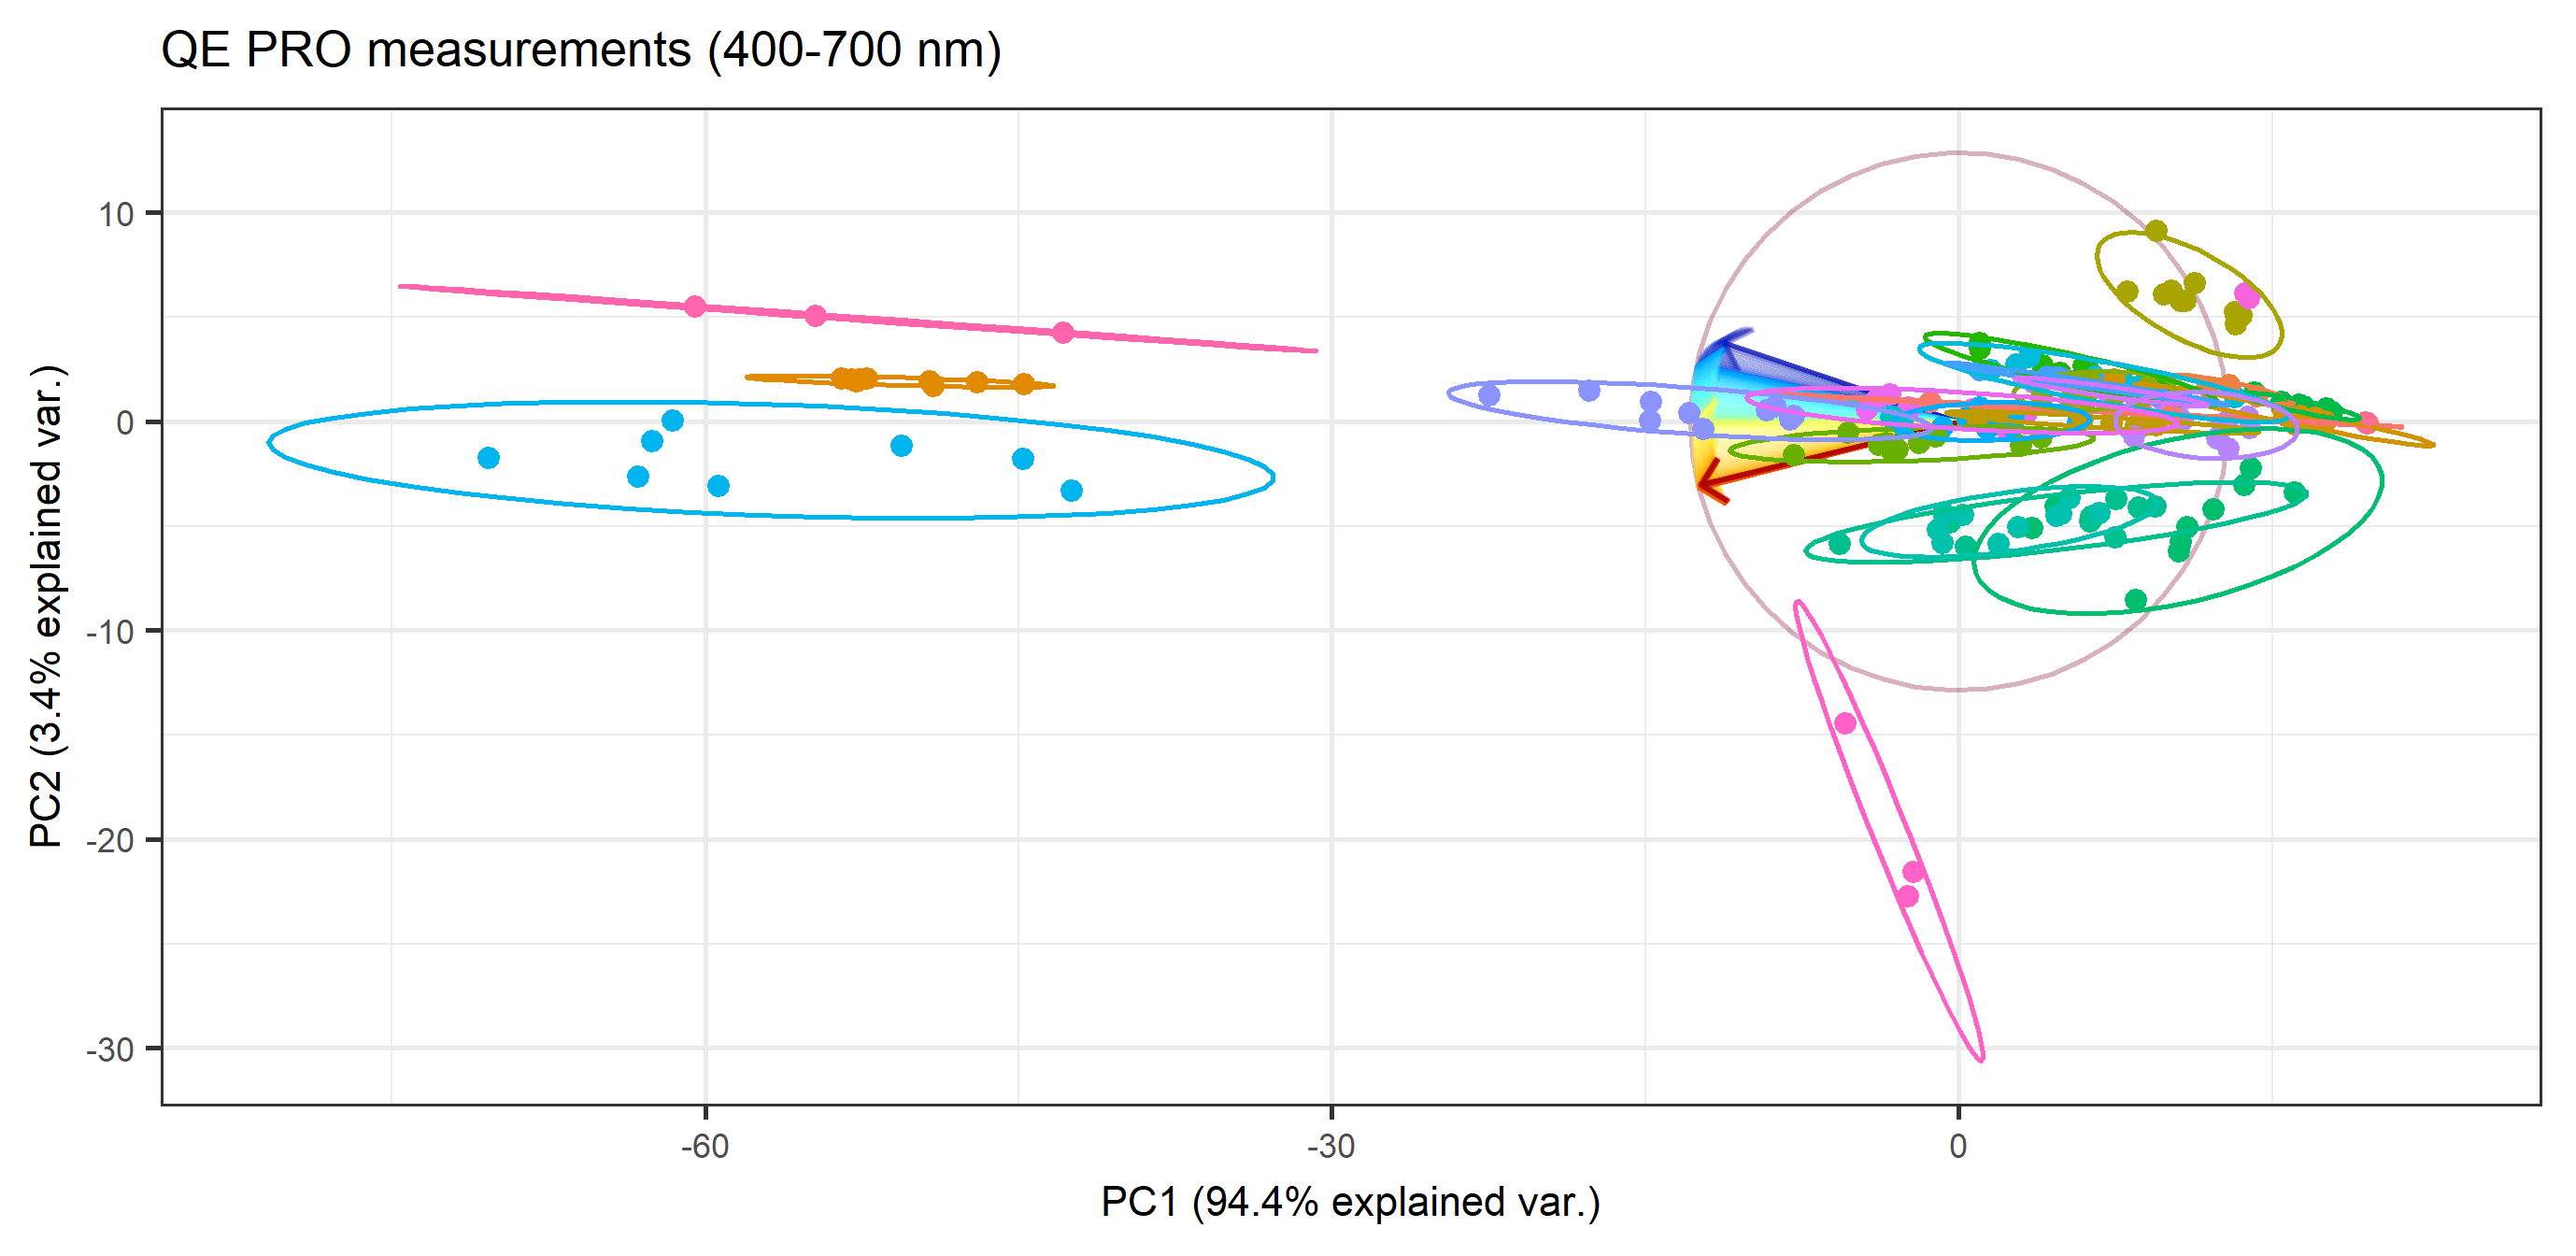
\includegraphics[width=1\textwidth]{Images/results/PCA_plastics_full_only_scat.png}
    \caption{Scatter plot of the results of the PCA with all plastic samples}
    \label{fig:PCA_plastics_only_full_scat}
\end{figure}


\begin{figure}[H]
   \centering
    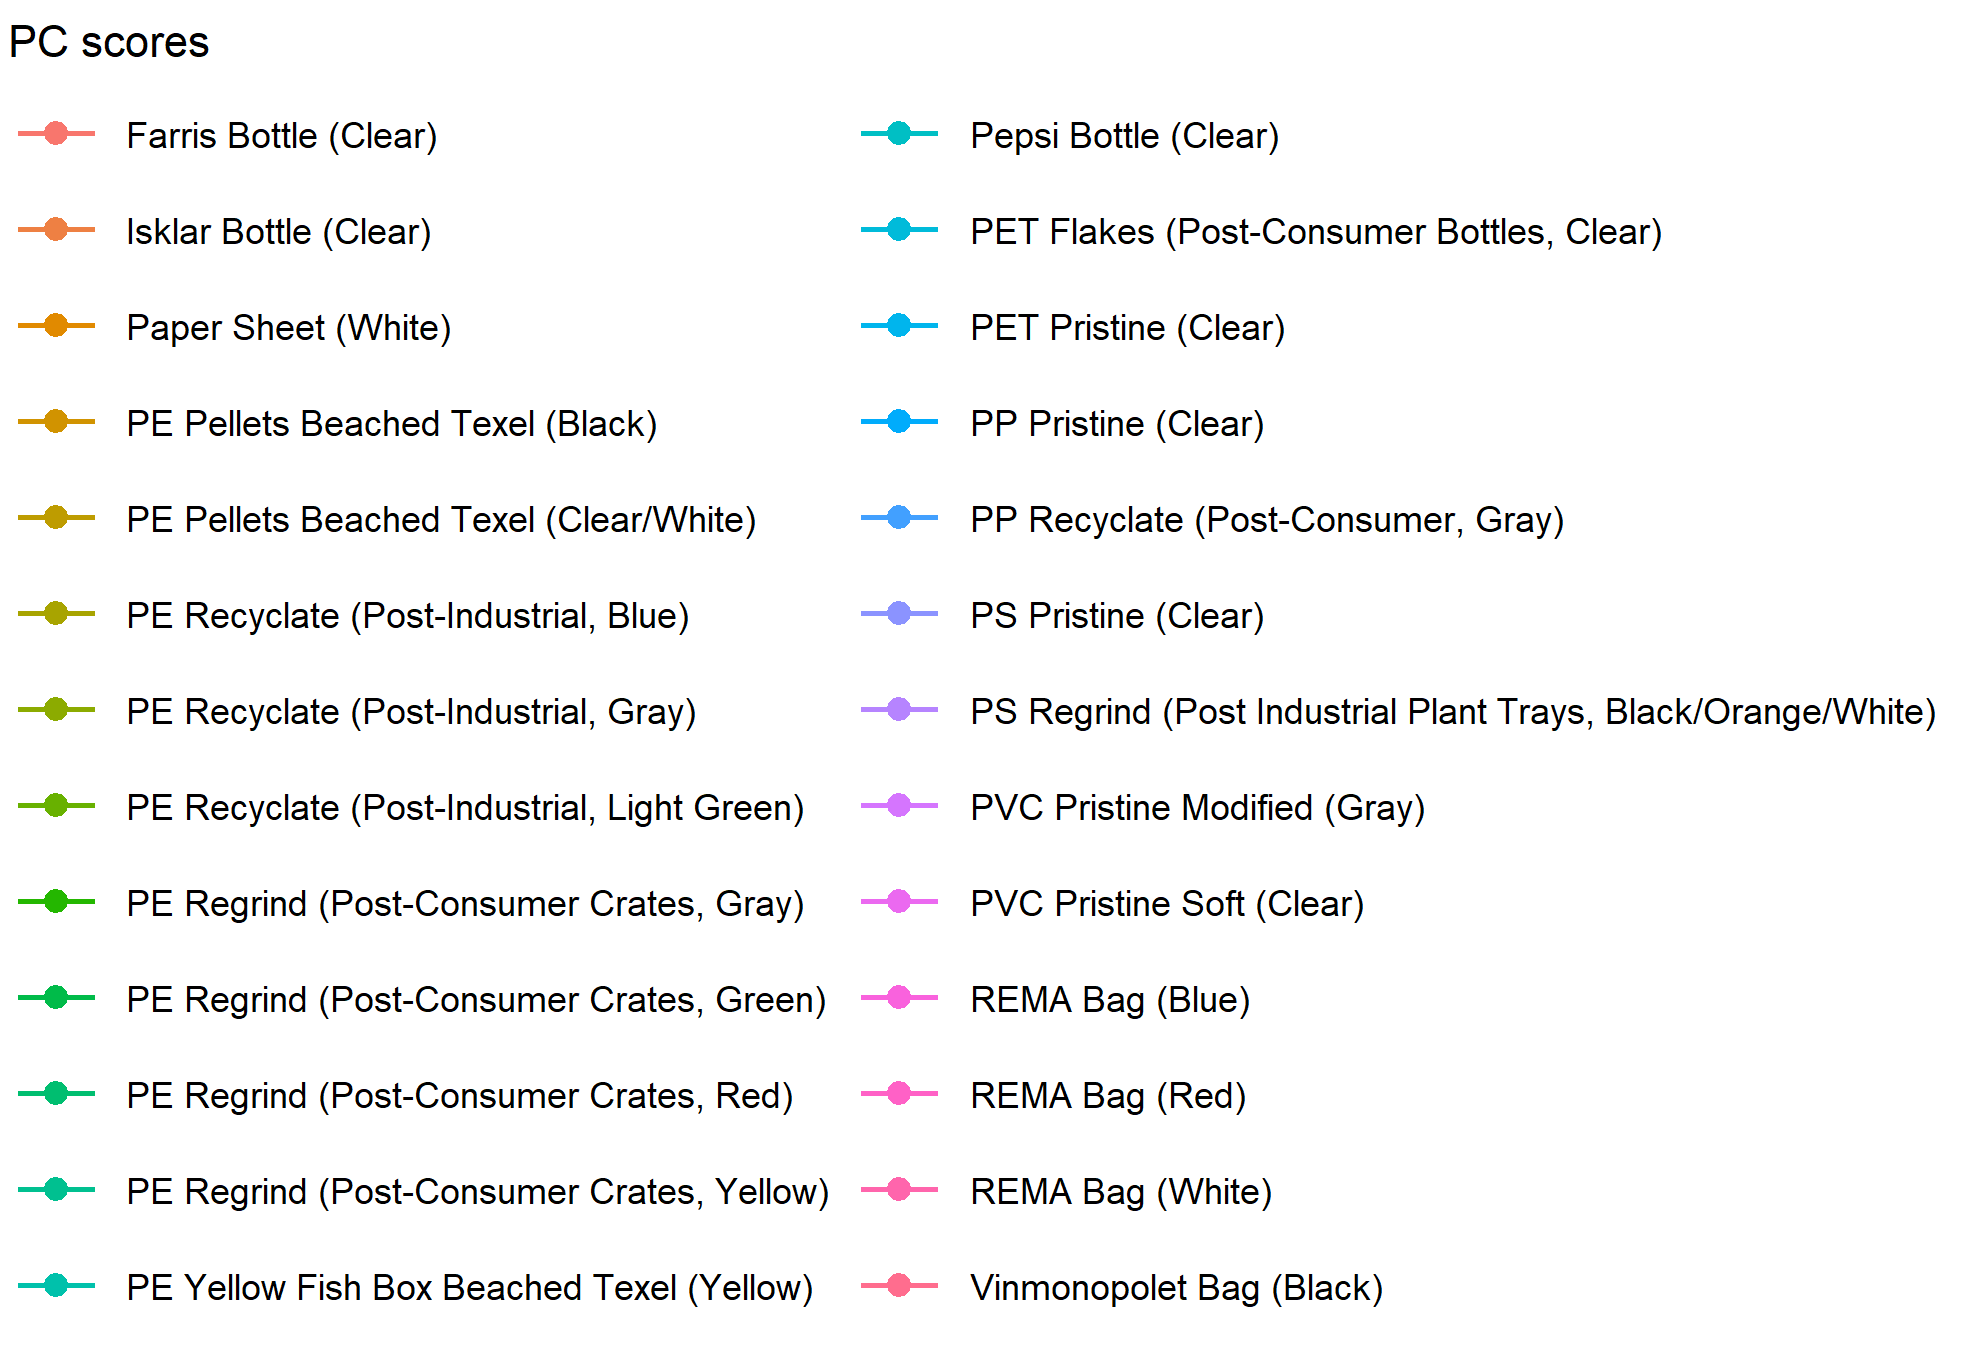
\includegraphics[width=0.7\textwidth]{Images/results/PCA_plastics_full_list.png}
  \caption{List of all scanned plastic samples and their respective colors.}
  \label{fig:PCA_plastics_full_list}
\end{figure}
\\\\
\noindent
As can be seen of the plot in Figure \ref{fig:PCA_plastics_only_full_scat}, PC1 accounts for over 94.1\% of the variance, while PC2 explains no more that 3.4\% of the variance. Interpreting the plot, there are three clustrings utenfor.. hvorfor? pga tynnhet og papiret. Velger å redusere ved å fjerne outliers vi ikke kan forklare fordi de har samme lyshet, farge og type som flere av de som ligger inne. Det resulterende sette, etter removal of outlying variables, presenteres i neste section.
\\\\
Figure \ref{fig:PCA_plastics_full_doub_cont} shows the contributions from the different wavelengths corresponding with the two principal components. The horizontal axis represent the wavelengths and the vertical axis the contribution in percent. The dashed red line represent 0.253\% or the line that shows the exact equal contribution from all wavelengths. Integrating the line would result in $0.253\% \cdot (700 - 400)/(0.758) \approx 100\%$.%Dette er feil. det skal være 0.252 siden det er en måling hver 0.758 og ikke hver nanometer, så er det mer riktig på bildet.
Also, the color of the line depicts the color at that wavelength, the blue color of the line at 450 nm is the color of light with that specific wavelength. 
\\\\%Påpeke at selv der man ser clusters så er ikke dette fremtredende i den samme plasttypen, men heller på bakgrunn av den fargen plasten innehar. 
\begin{figure}[H]
    \centering
    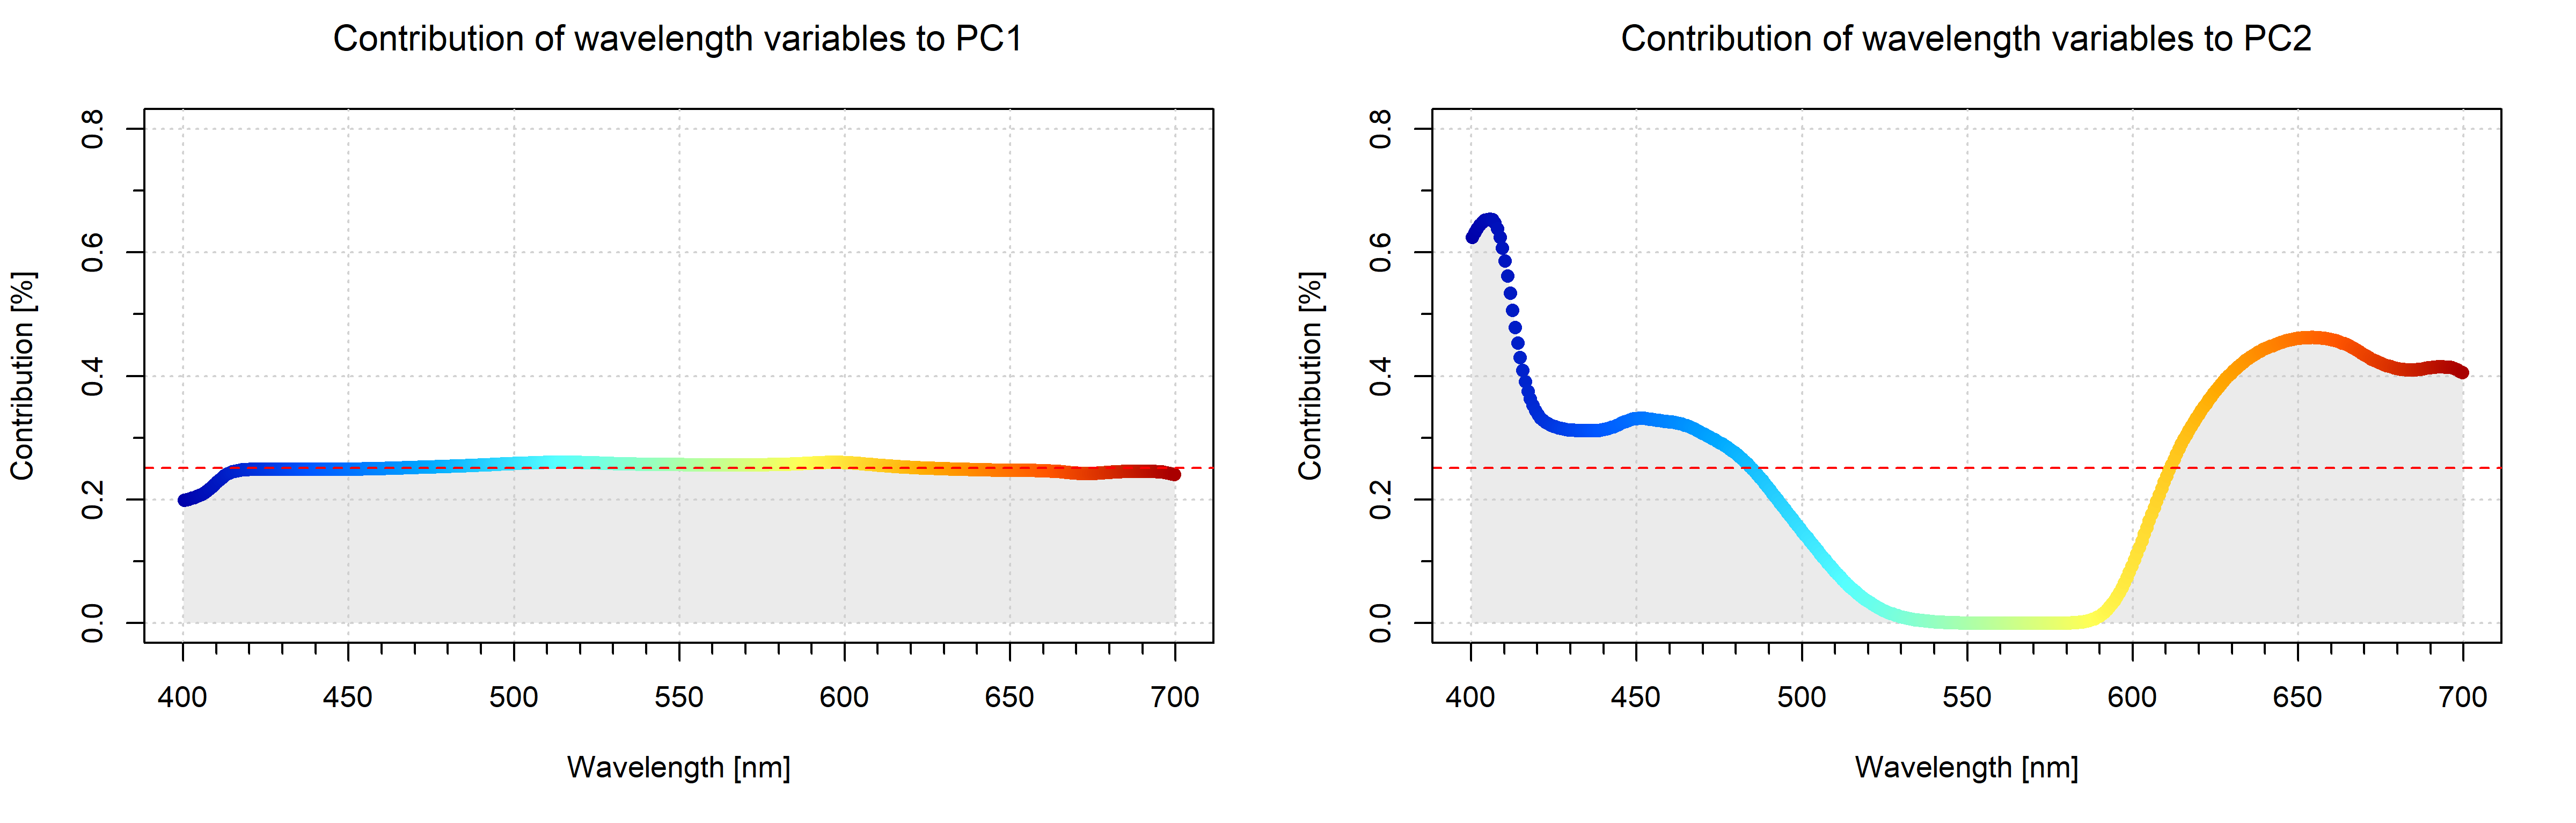
\includegraphics[width=1\textwidth]{Images/results/PCA_plastics_full_doub_cont.png}
    \caption{Contribution plot of the results of the PCA with all plastic samples.}
    \label{fig:PCA_plastics_full_doub_cont}
\end{figure}
\noindent
From the signature and contribution of PC1 in Figure \ref{fig:PCA_plastics_full_doub_cont} it is apparent that the 94.1\% descriptive property of the first principal component is not rooted in one wave length or in a combination of wavelengths. The even distribution over the spectrum visualize the fact that PC1 mainly describes the \textit{lightness} of the plastic. 
\\\\
In addition, the position of the different samples in Figure \ref{fig:PCA_plastics_only_full_scat}, also indicate that the results are dominated by this fact. Due to the low variance of the second principal component, of only 3.4 \%, the vertical spread and thus the few clusters there are, are not well described and may not be deemed representative.
\\\\

\subsection{Principal Component Analysis with Reduced Plastic Samples}
As explained in the previous section, the results presented in this section are from a reduced dataset. Based on the knowledge provided through analyzing the results of the full set, some variables was removed. This way, the reduced set contains only relevant redeemed variables without wrongly measured samples possibly pulling the result in the wrong direction. 
\\\\
Figure \ref{fig:PCA_plastics_reduced_only_scat} is the scatter plot describing this reduced set. The properties of this scatter plot are the same as for the scatter plot presented for Figure \ref{fig:PCA_plastics_only_full_scat} in Section \ref{sec:pcafull}, and will therefore not be elaborated here as well.

\begin{figure}[H]
    \centering
    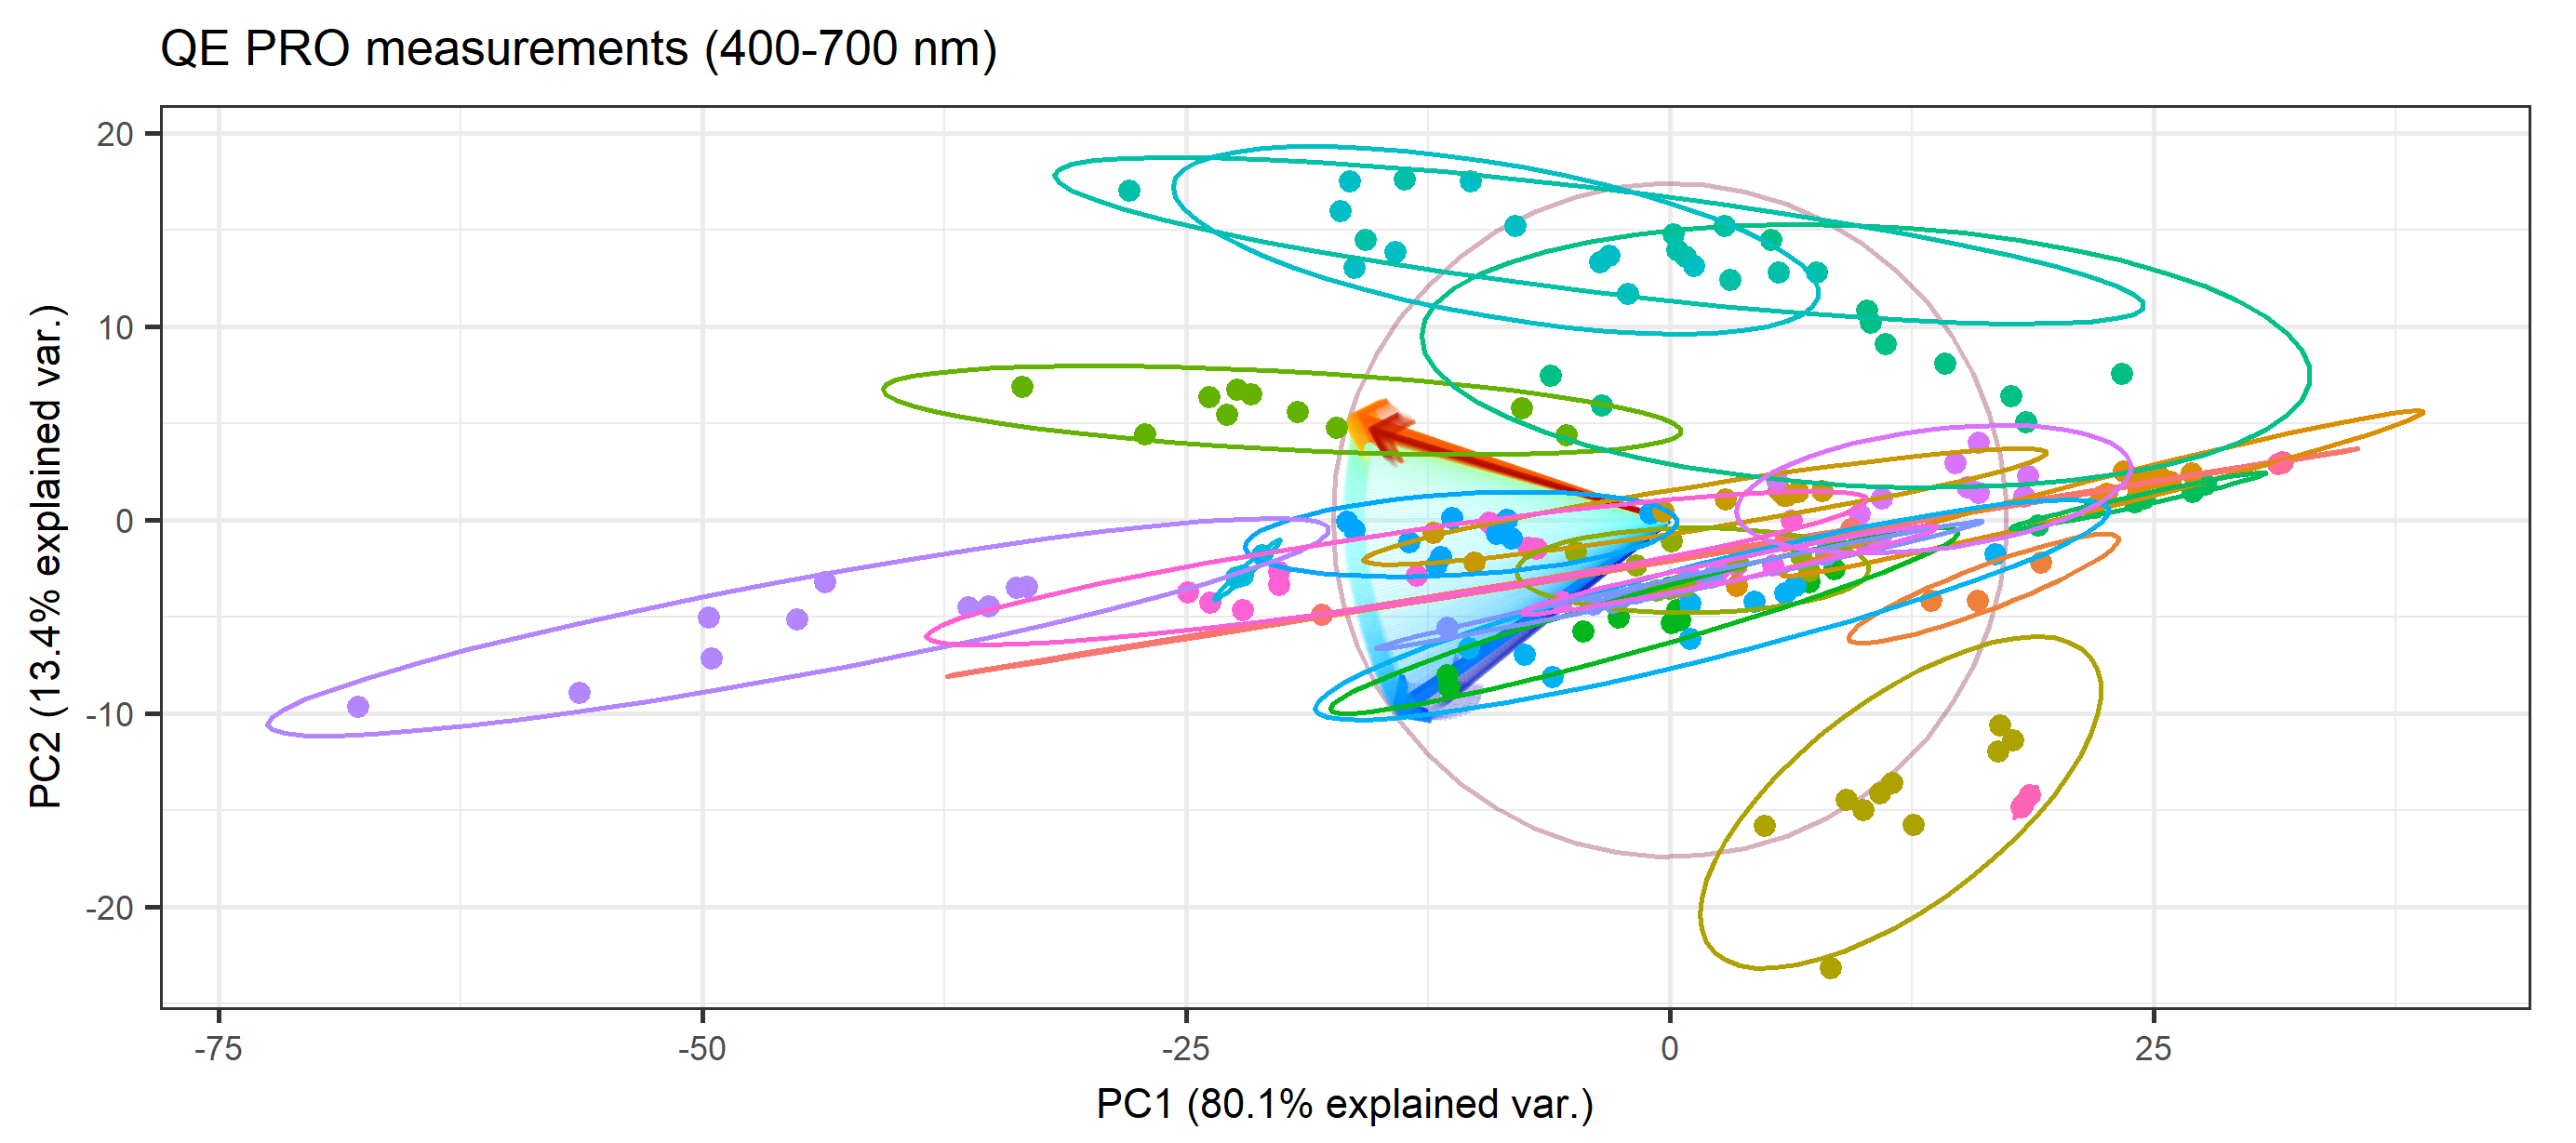
\includegraphics[width=1\textwidth]{Images/results/PCA_plastics_reduced_only_scat.png}
    \caption{Results of the PCA with reduced Plastic Samples}
    \label{fig:PCA_plastics_reduced_only_scat}
\end{figure}

\begin{figure}[H]
    \centering
    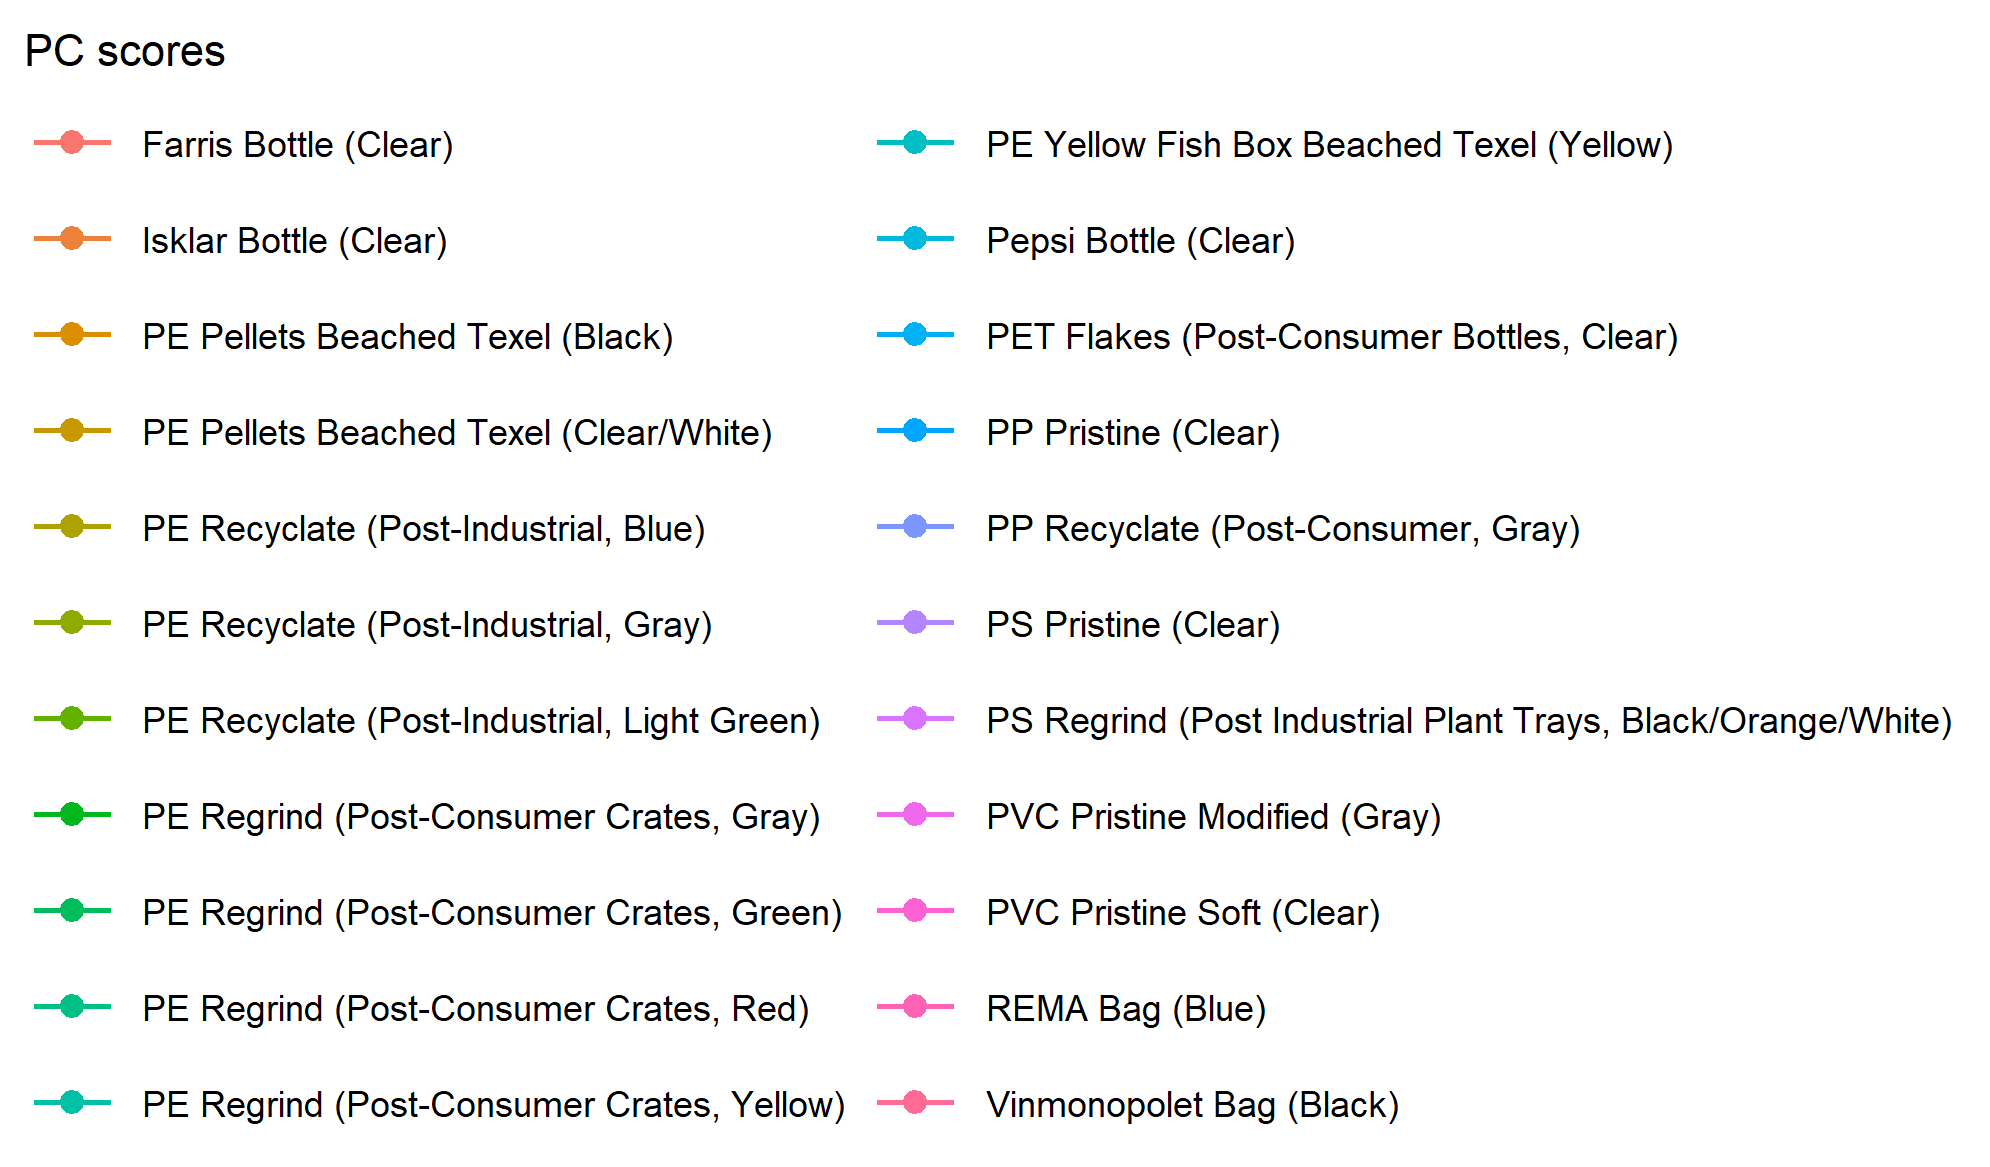
\includegraphics[width=0.7\textwidth]{Images/results/PCA_plastics_reduced_list.png}
    \caption{List of the reduced scanned plastic samples and their respective colors.}
    \label{fig:PCA_plastics_reduced_list}
\end{figure}
\noindent
PC1 now represents 80.1\% of the variance, while PC2 explains 13.4\% of the variance. Despite the lower explanation percentage of PC2, there are clusters. These are quite apparent in the top and bottom of the scatter plot (\ref{fig:PCA_plastics_reduced_only_scat}). The issue arise when comparing these clusters to their respective plastic type. There are no other clear clusters related to these types of plastic. In fact, it seems that the clear clusters these types are a part of, are based on the color of the plastic, not inherent properties of the material. The bottom cluster consists of PE Recyclate of the color blue together with samples retrieved from the blue part of the logo on a plastic bag. Similarly, the top cluster consists of PE Regrind and PE Yellow Fish Box Beached Texel, both of which are yellow-colored. It is therefore difficult to argue that these clusters indicate anything other than the color additives in the material.
\\\\
%Tenke på å markere clusterene med tall, slik at det blir lettere å omtale
Based on the tendency of the clear plastic to be on the left side of the cluster, one can assume that the white paper background have had an impact on the results, and subsequently on the principal components. The samples of PS Pristine were particularly clear, as may be seen from the table in the Section \ref{sec:material} in Chapter \ref{chap:method}, or as an image in Appendix \ref{app:image_plast}. Given that these are the main contributions to the spread along the horizontal axis, one could argue that without the light background, the lightness and clearness of the material would be less prominent in the first principal component. This would possibly further change the composition of the principal components and subsequently change the patterns on the scatter plots. 
\\\\%Snakke med Asgeir om dette og høre hva han tenker om at papiret har påvirket resultatene og at vi i utgangspunktet ikke har tid til å tilbringe en hel ny dag på laben for å teste på nytt. Aksel har gjort tester tidligere der han har fått samme resultat med at "lysheten" til prøvene har hatt stor innvirkning
\noindent
The associated contribution plot is displayed in Figure \ref{fig:PCA_plastics_doub_cont}. This plot show how the different wavelength contribute in correspondence to PC1 and PC2, respectively. 

\begin{figure}[H]
    \centering
    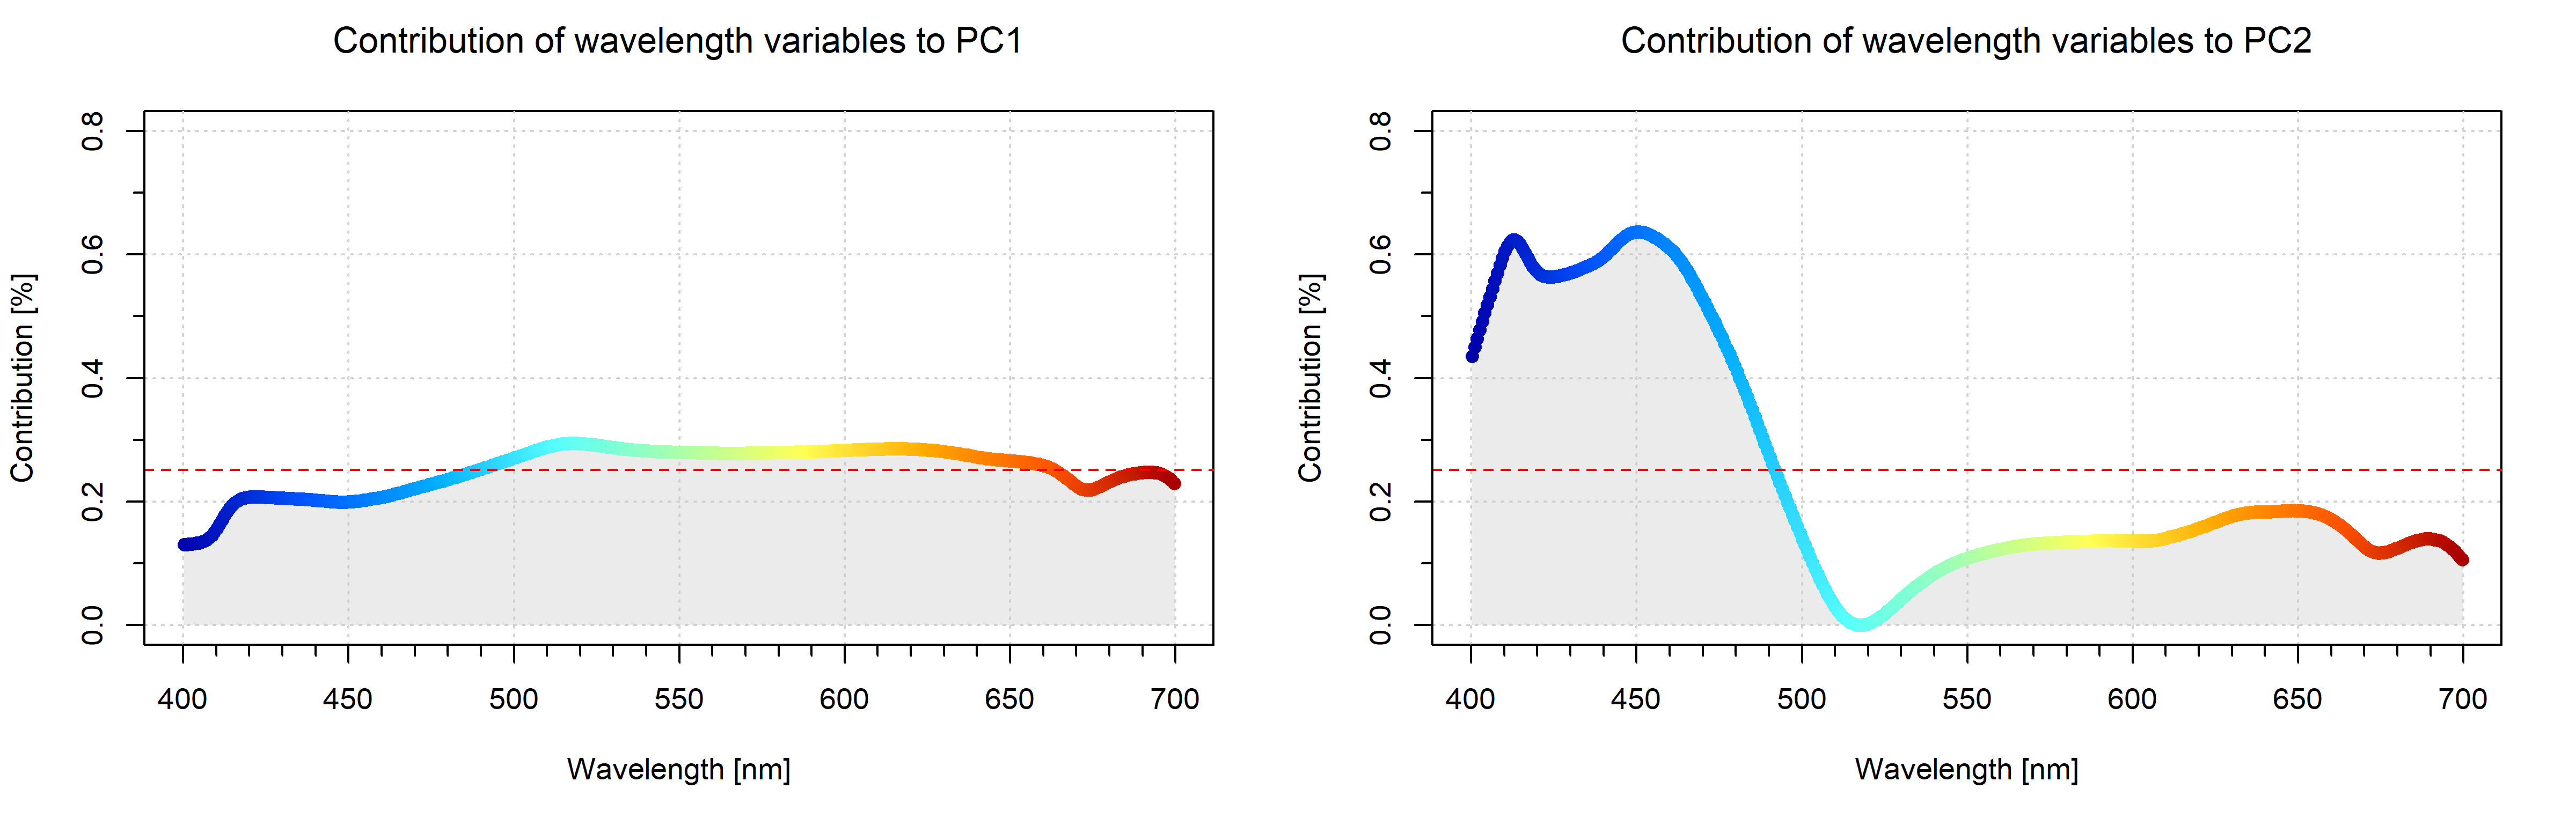
\includegraphics[width=1\textwidth]{Images/results/PCA_plastics_reduced_doub_cont.png}
    \caption{Contribution plots of the two principal components of the PCA with reduced plastic samples}
    \label{fig:PCA_plastics_doub_cont}
\end{figure}
\noindent
The contribution plot of the second principal component imply that the lower end of the spectrum has ha larger impact than the larger wavelengths. 

\subsection{Principal Component Analysis with Biological Components}
Figures \ref{fig:PCA_plastics_and_biology_scat} and \ref{fig:PCA_and_bio_cont_plots} are plots describing the results of plastic samples together with biological pigments - initially presented at the end of Chapter \ref{chap:method}. These plots have the same properties as those above, solely consisting of plastic.

\begin{figure}[H]
    \centering
    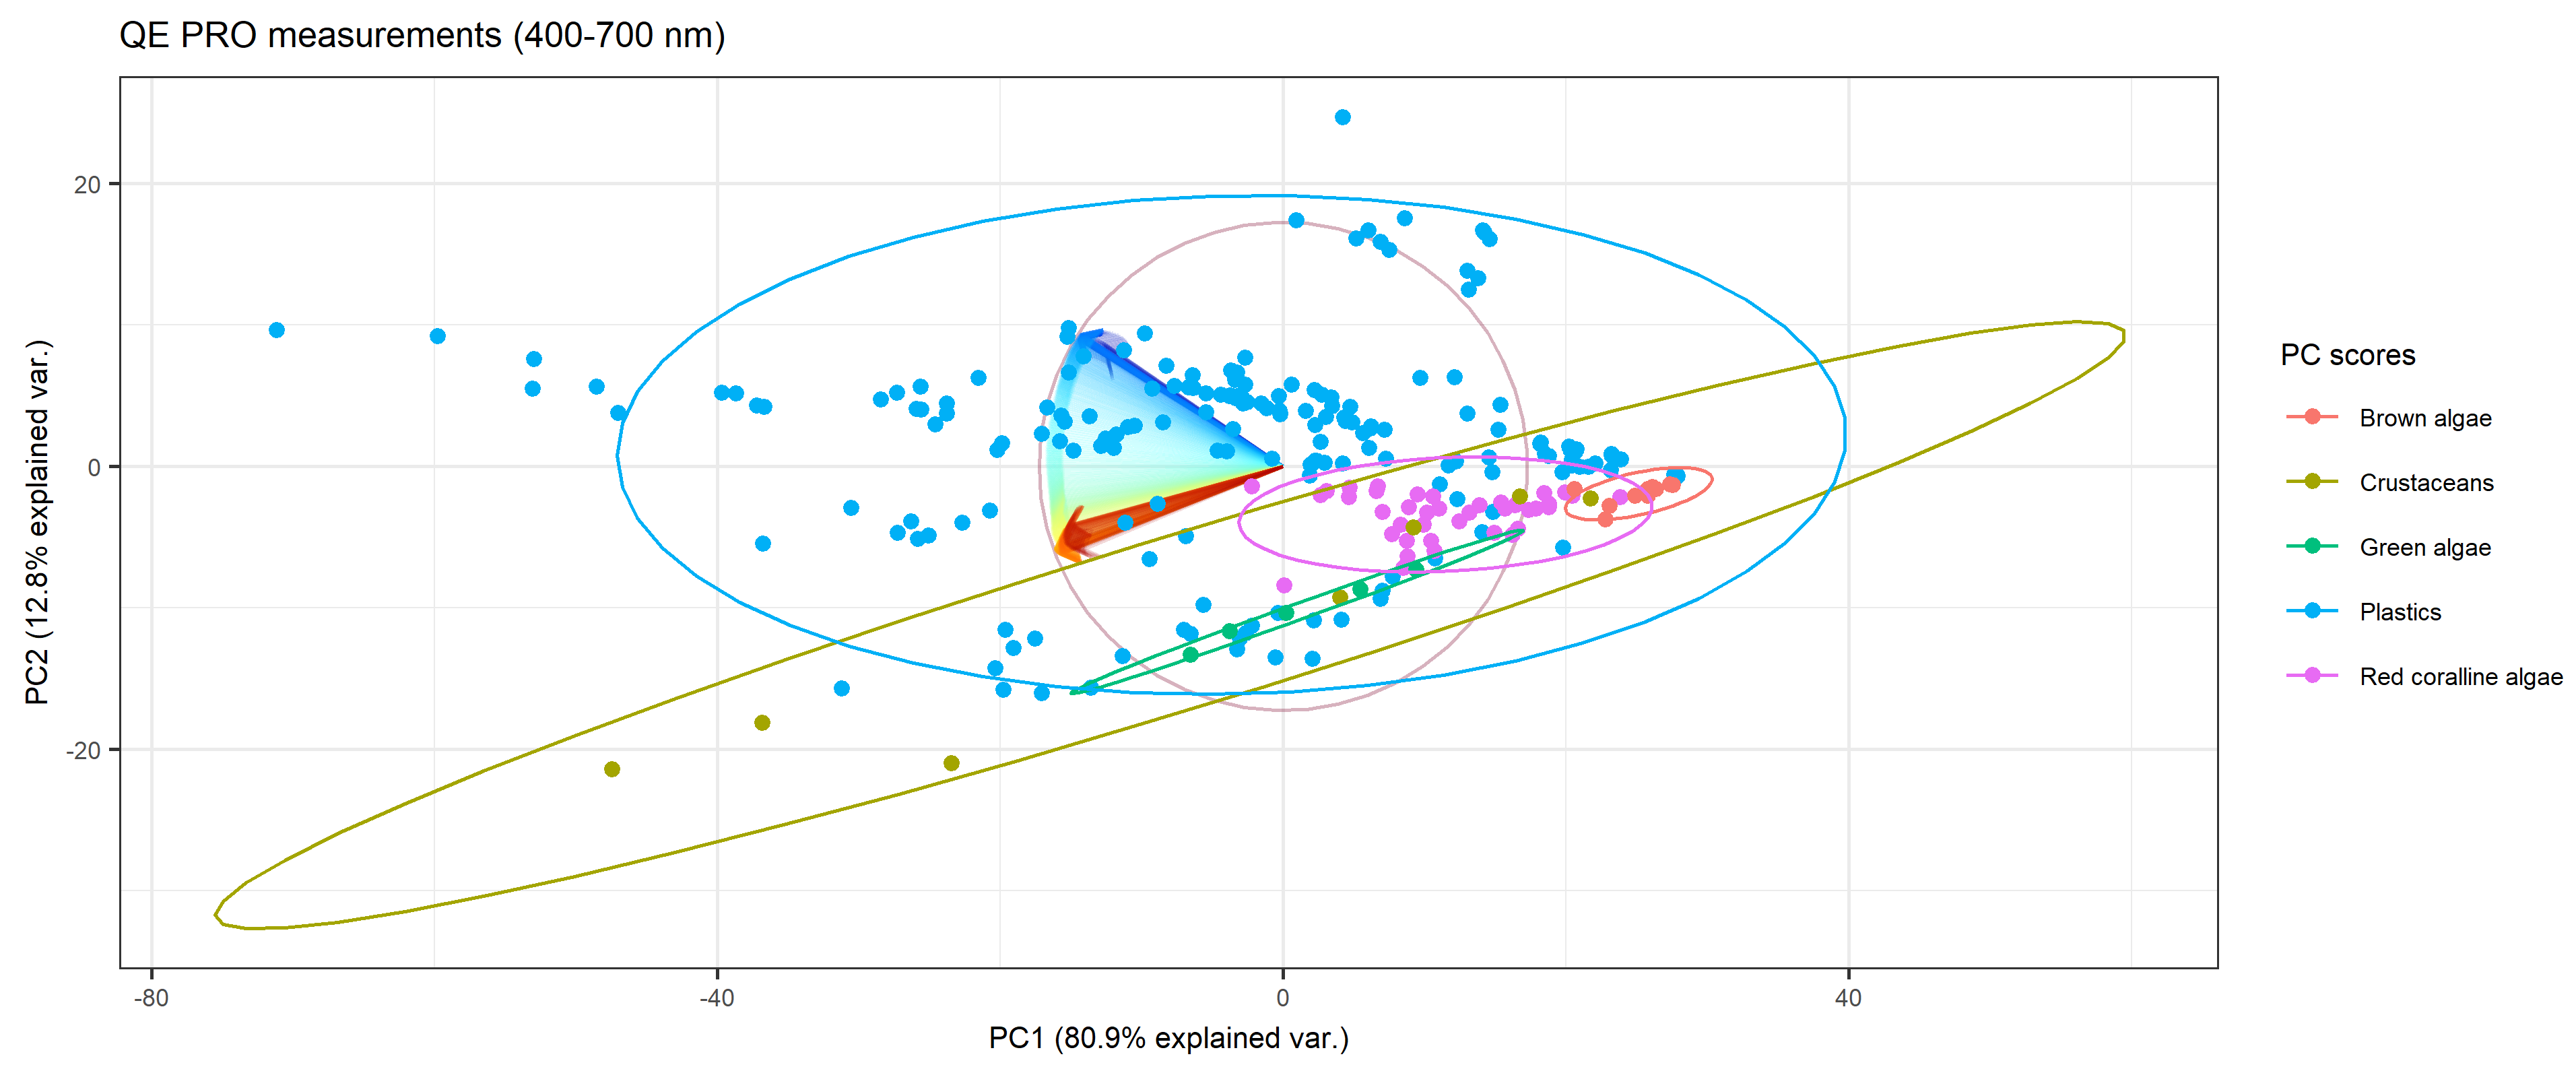
\includegraphics[width=1\textwidth]{Images/results/PCA_plastics_and_biology_scat_clust.png}
    \caption{Results of the PCA with Plastics and Biological Components}
    \label{fig:PCA_plastics_and_biology_scat}
\end{figure}


\begin{figure}[H]
  \newcommand*\FigVSkip{0.5em}
  \newcommand*\FigHSkip{0.1em}
  \newsavebox\FigBox
  \centering
  % Top image is centered, so no need to get width
 \sbox{\FigBox}{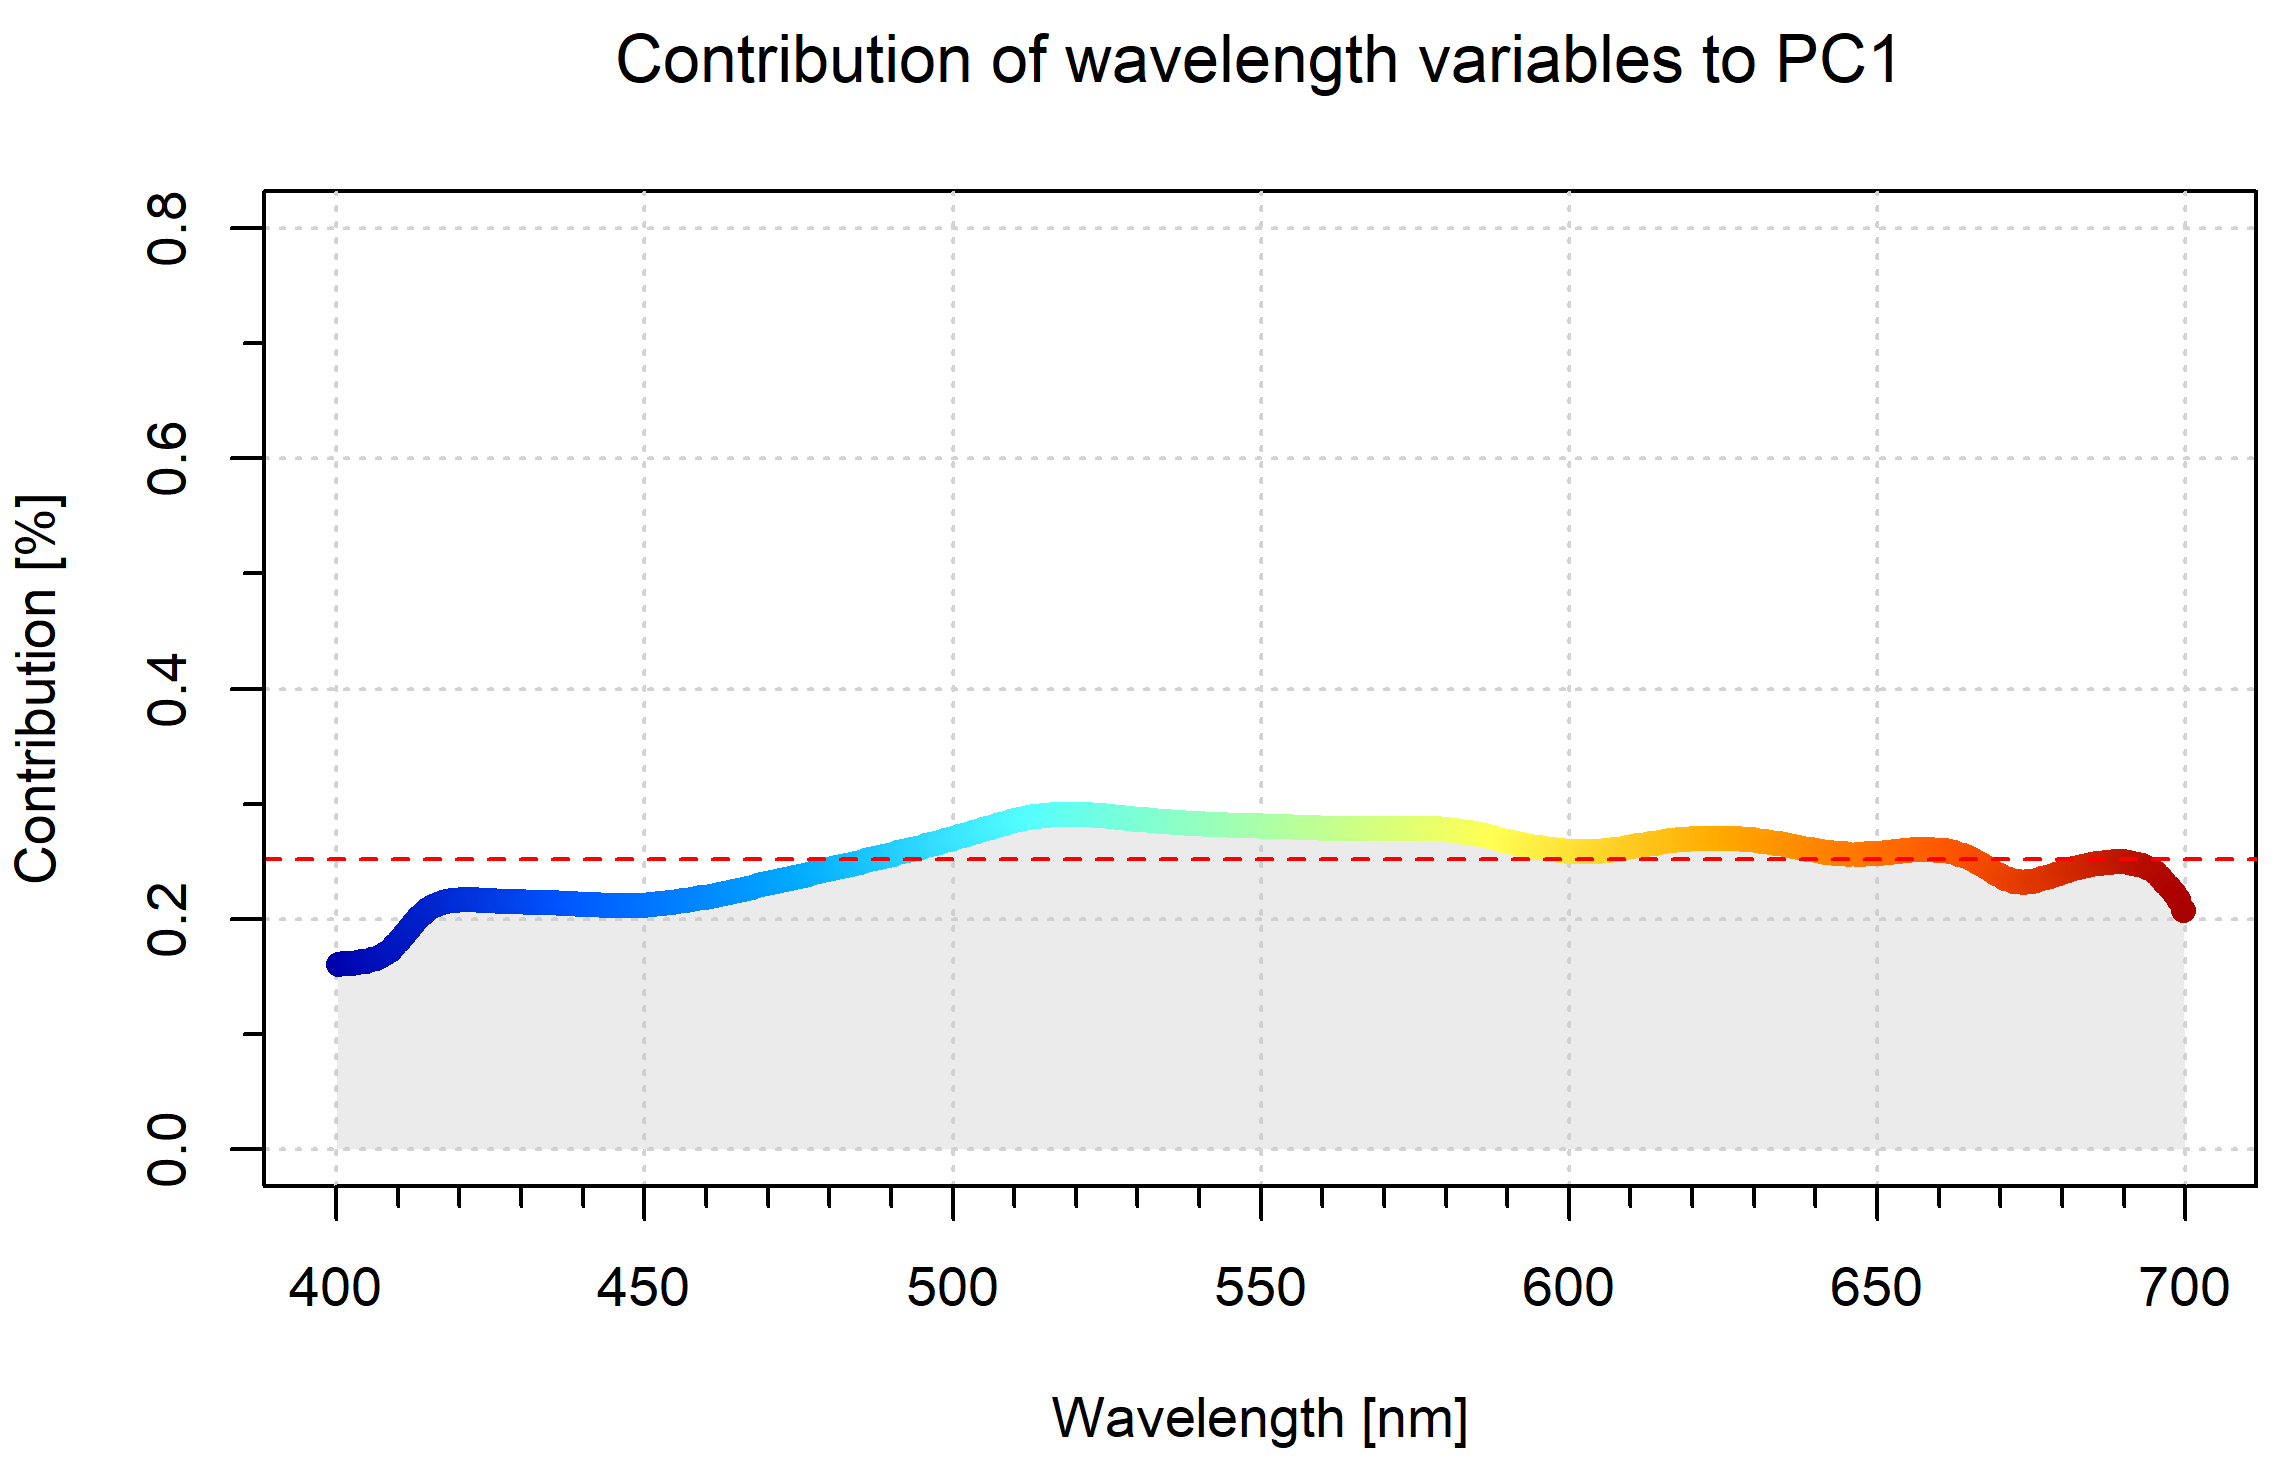
\includegraphics[scale=0.5]{Images/results/PCA_plastics_and_biology_cont_pc1.png}}
  \begin{minipage}{\wd\FigBox}
    \centering\usebox{\FigBox}
     \label{fig:PCA_plastics_and_biology_cont_pc1}
  \end{minipage}
    % Top image is centered, so no need to get width
 \sbox{\FigBox}{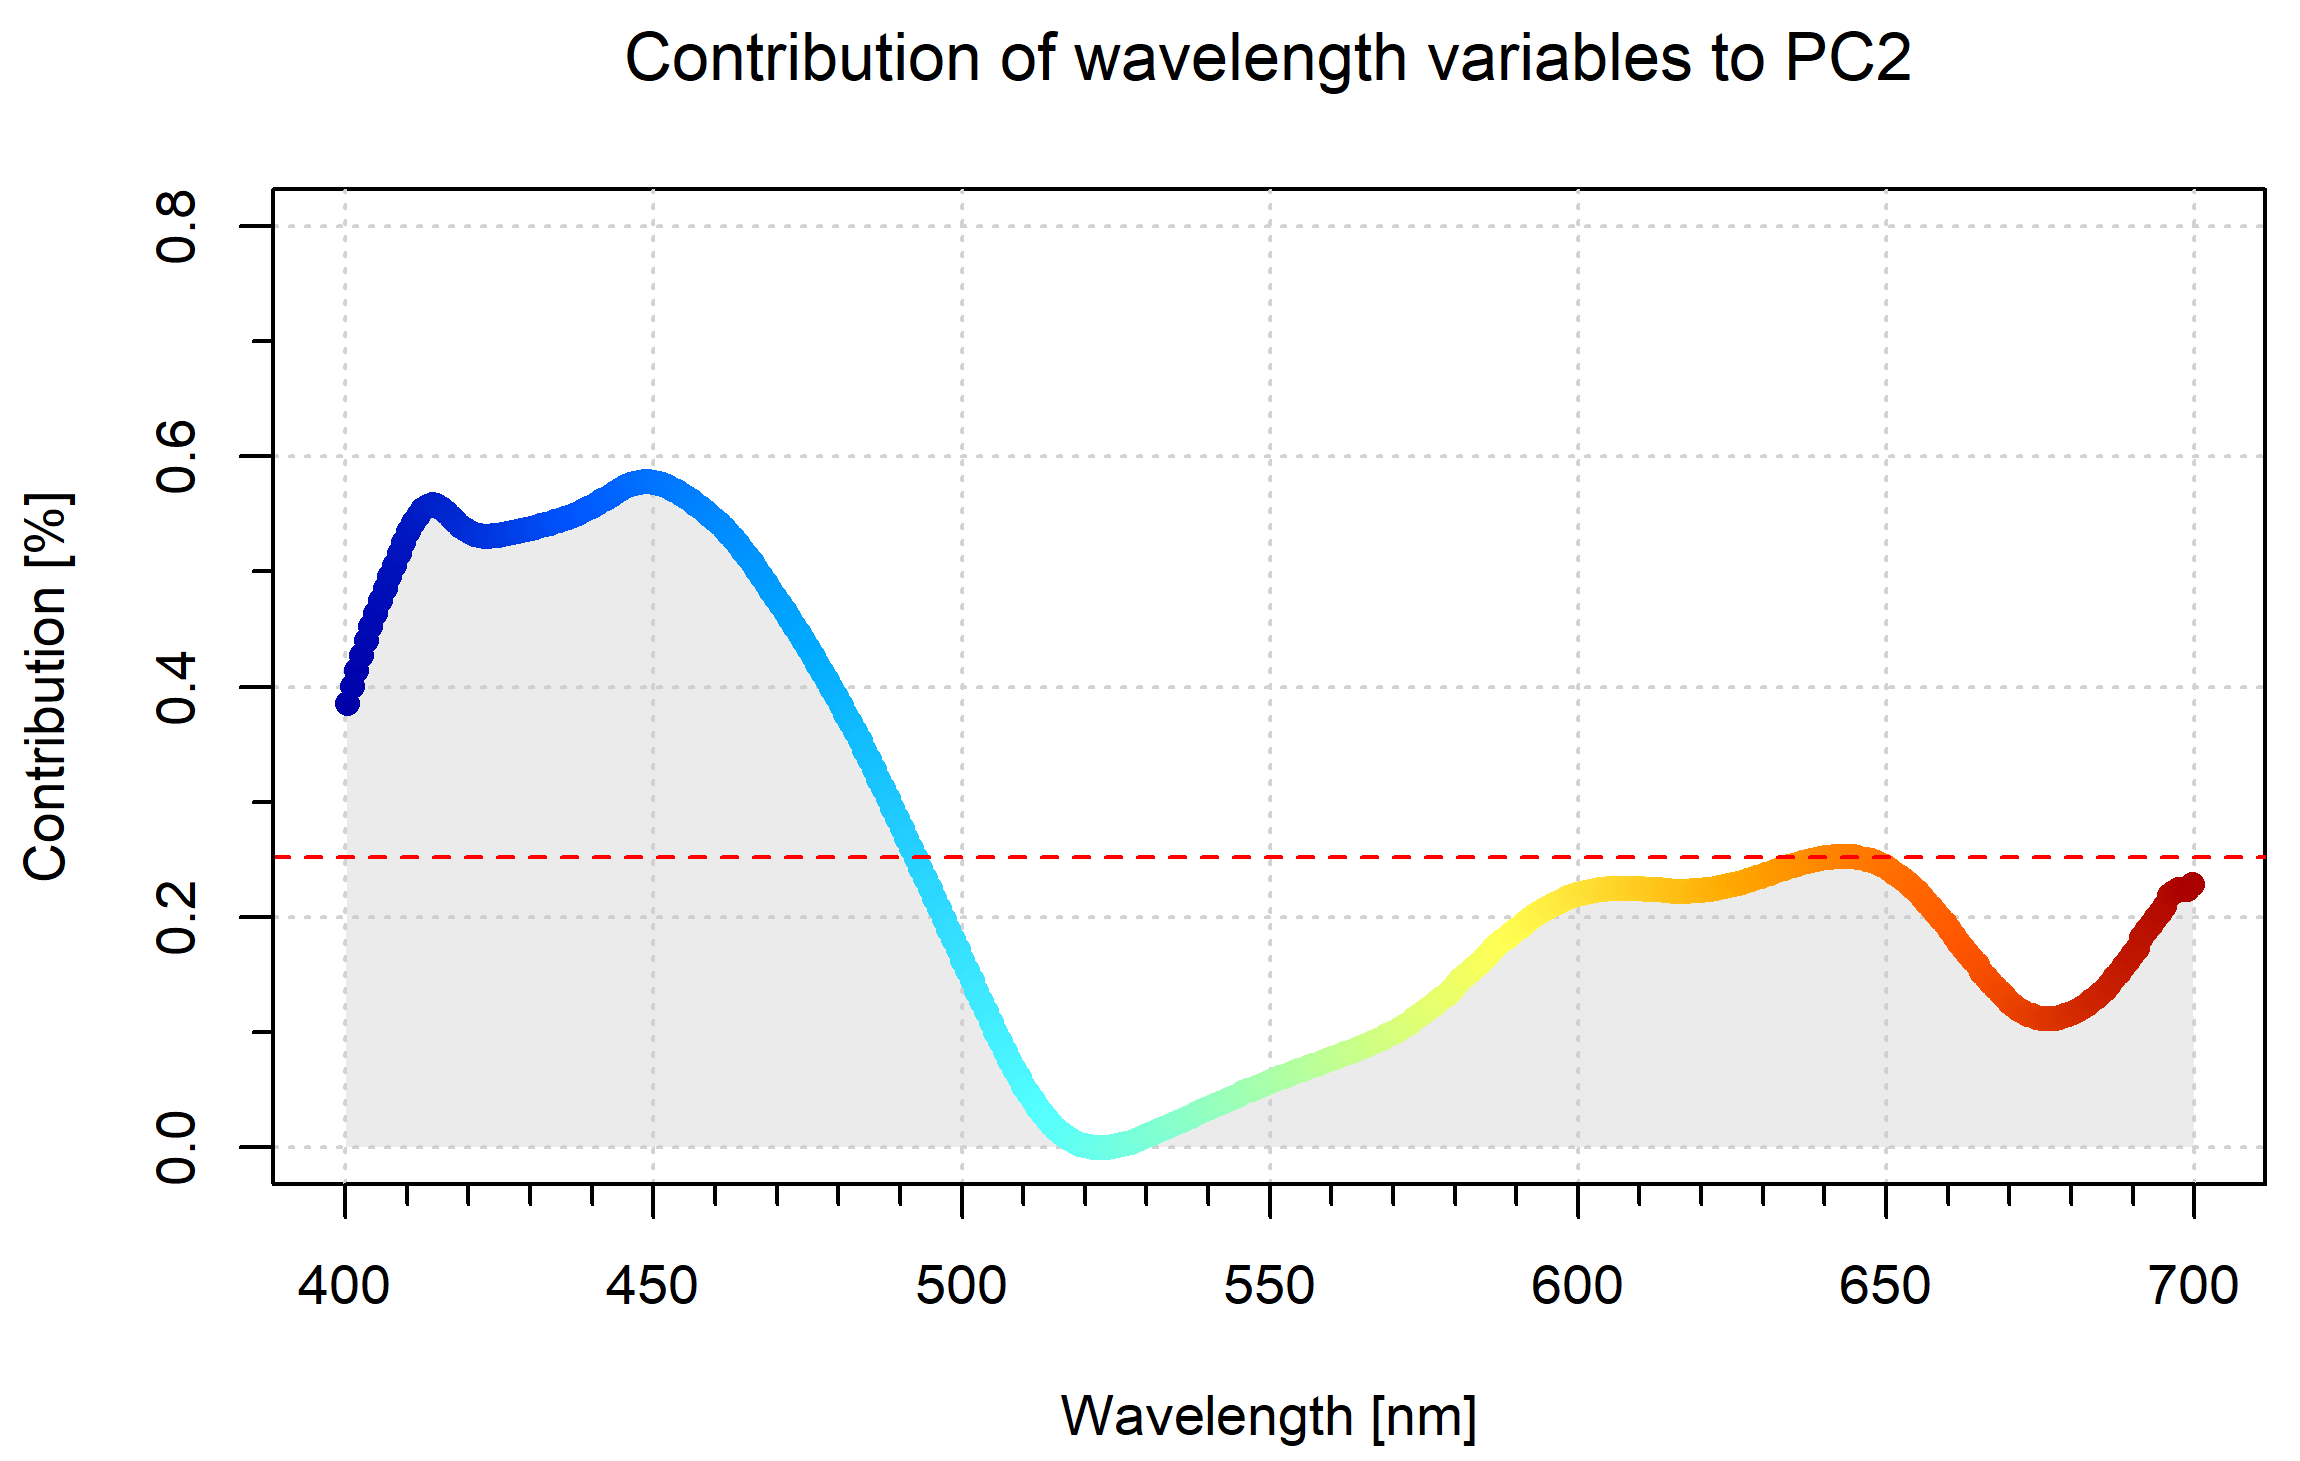
\includegraphics[scale=0.5]{Images/results/PCA_plastics_and_biology_cont_pc2.png}}
  \begin{minipage}{\wd\FigBox}
    \centering\usebox{\FigBox}
  \label{fig:PCA_plastics_and_biology_cont_pc2}
  \end{minipage}
  % Save second image 
  \caption{Contribution plots for the PCA with plastic and biological samples}
\label{fig:PCA_and_bio_cont_plots}
\end{figure}
\noindent
Interpreting these figures, a more prominent trend became apparent. The natural occurring pigment in algae and crustaceans differed from the plastic in the scatter plot. This shows potential for distinguishing plastic in general from organic pigments naturally occurring in the marine environment.
\\\\%Argumentere med at her ser man at den klare plasten ligger utenfor konfidens intervallet og kan dermed mulig ekskluderes i en ny runde med forsøk, eventuelt at man endre bakgrunnen slik at den ikke er hvit og dermed ikke påvirker lysheten i tilsvarende grad. 
The contribution on the first principal component does not differ much from the associated components in the previous plots. However, given the mentioned effect of the clear plastic, this might change with the use of a less reflective background. Furthermore, in Figure \ref{fig:PCA_plastics_and_biology_scat} all plastic samples are gathered in one confidence interval ring. The result is that the previously mentioned clear plastic lies outside the confidence interval. This would further underline the previous suspicion that there is a prominent effect from the white background on the results.
\\\\
Experience has shown that the brightness/lightness of the samples is highly relevant also when not investigating plastic. Therefore, the change in background might affect the results, but it is not expected to revolutionize them.
\\\\\\
Now, what can be drawn of this? Acquiring distinct signatures for the specific types of plastic, seems unlikely using a hyperspectral image. Neither was is possible to find a general signature for the plastic, increasing the difficulty of detecting plastic as a total. %which could be used as an end-member or for Spectral Angle Mapping. 
\\\\
Despite seeing a resemblance of a signature in the second principal component it is important to keep in mind the components do not represent actual signatures. They rather depict the wavelengths which have a larger influence on the vertical distinguishing of the samples.
\\\\
Based on the absence of clear clusters it was deemed not possible to acquire what is thought of as unique signatures for the plastic. All three analyses do show vertical spread, but the large number of overlapping samples made it difficult to argue for the existence of clear signatures at this stage. In the analysis with the presence of the organic pigments, there are some indication of separation, but not enough argue for a general signature for the plastic. However, the clustering seen in the sample does pose an opportunity of distinguishing plastic from the natural occurring pigments. 

\vspace{1.3cm}
\section{Signatures}

\subsection{Constant Color}
The resulting signatures were highly affected by the color of the targeted plastic pellets. Figure \ref{fig:plastcomp1}, shows the spectrum of two types, PP and PVC respectively. 

\begin{figure}[H]
  \newcommand*\FigVSkip{0.5em}
  \newcommand*\FigHSkip{0.1em}
  \newsavebox\FigBox
  \centering
  % Top image is centered, so no need to get width
 \sbox{\FigBox}{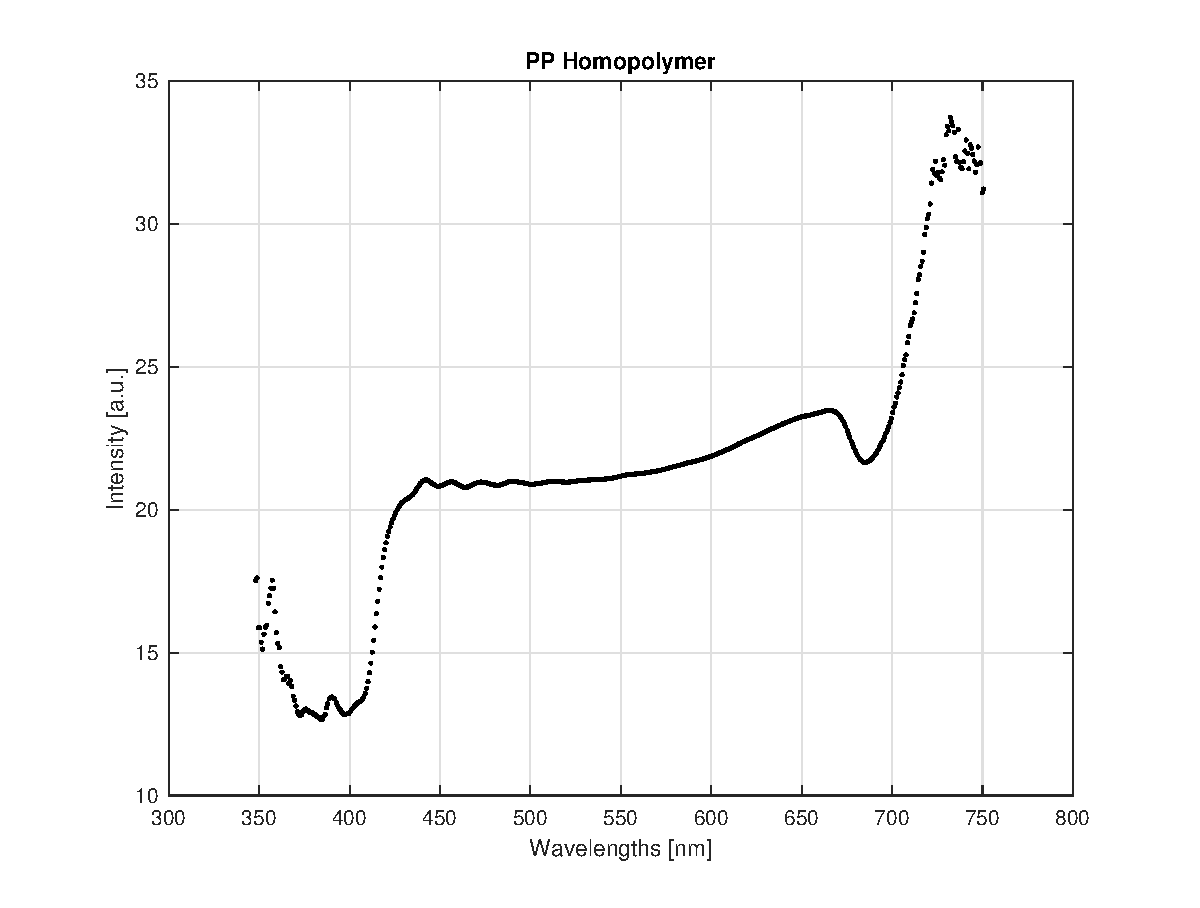
\includegraphics[scale=0.36]{Images/appendix/pp-pristine-clear.eps}}
  \begin{minipage}{\wd\FigBox}
    \centering\usebox{\FigBox}
    \subcaption{a) PP Pristine}
  \end{minipage}
    % Top image is centered, so no need to get width
 \sbox{\FigBox}{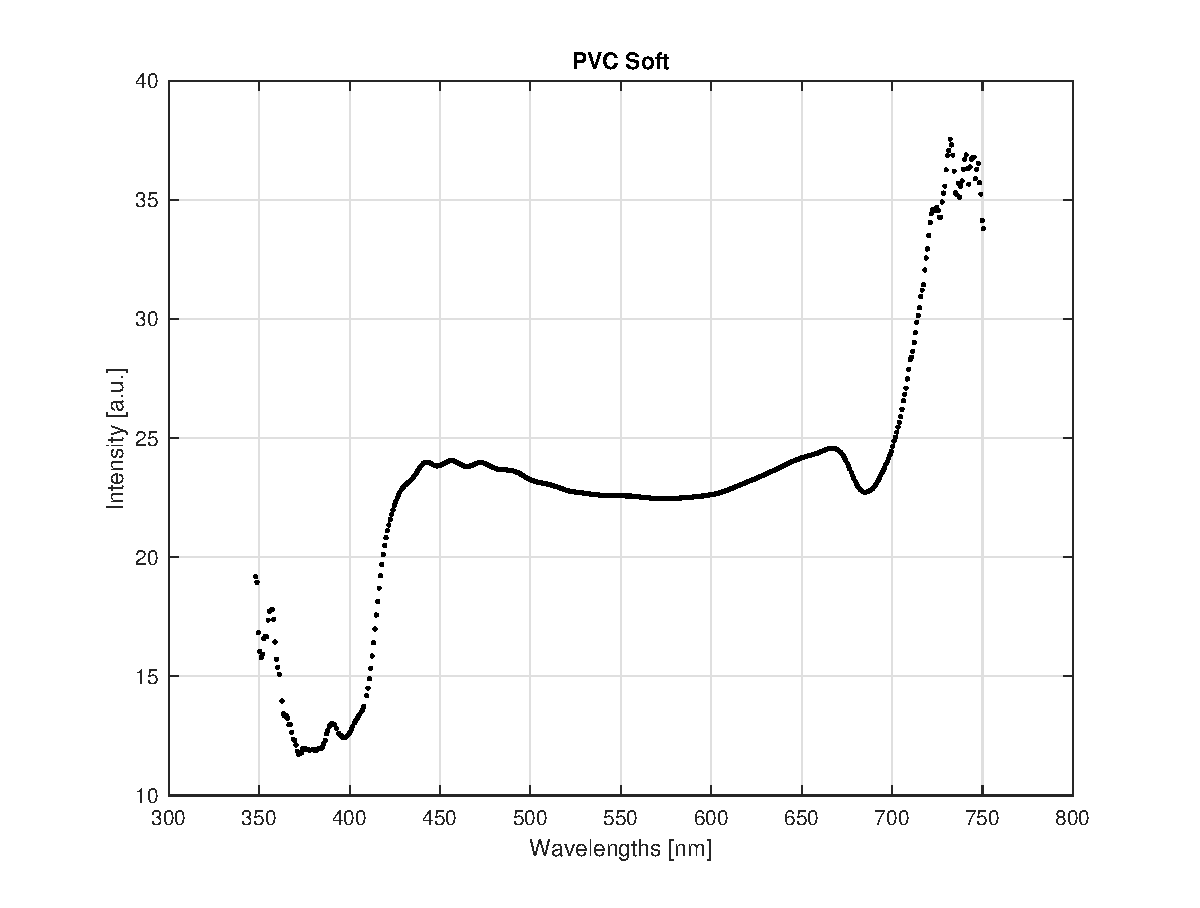
\includegraphics[scale=0.36]{Images/appendix/pvc-soft-pristine-clear.eps}}
  \begin{minipage}{\wd\FigBox}
    \centering\usebox{\FigBox}
    \subcaption{b) PVC Soft Pristine}
  \end{minipage}
  % Save second image 
  \caption{A comparison of the resulting signature for PP and PVC - both clear-colored}
  \label{fig:plastcomp1}
\end{figure}

%denne viser gule for pe og pe-hd, men de er kanskje for like..
\begin{comment}
\begin{figure}[H]
  \newcommand*\FigVSkip{0.5em}
  \newcommand*\FigHSkip{0.1em}
  \newsavebox\FigBox
  \centering
  % Top image is centered, so no need to get width
 \sbox{\FigBox}{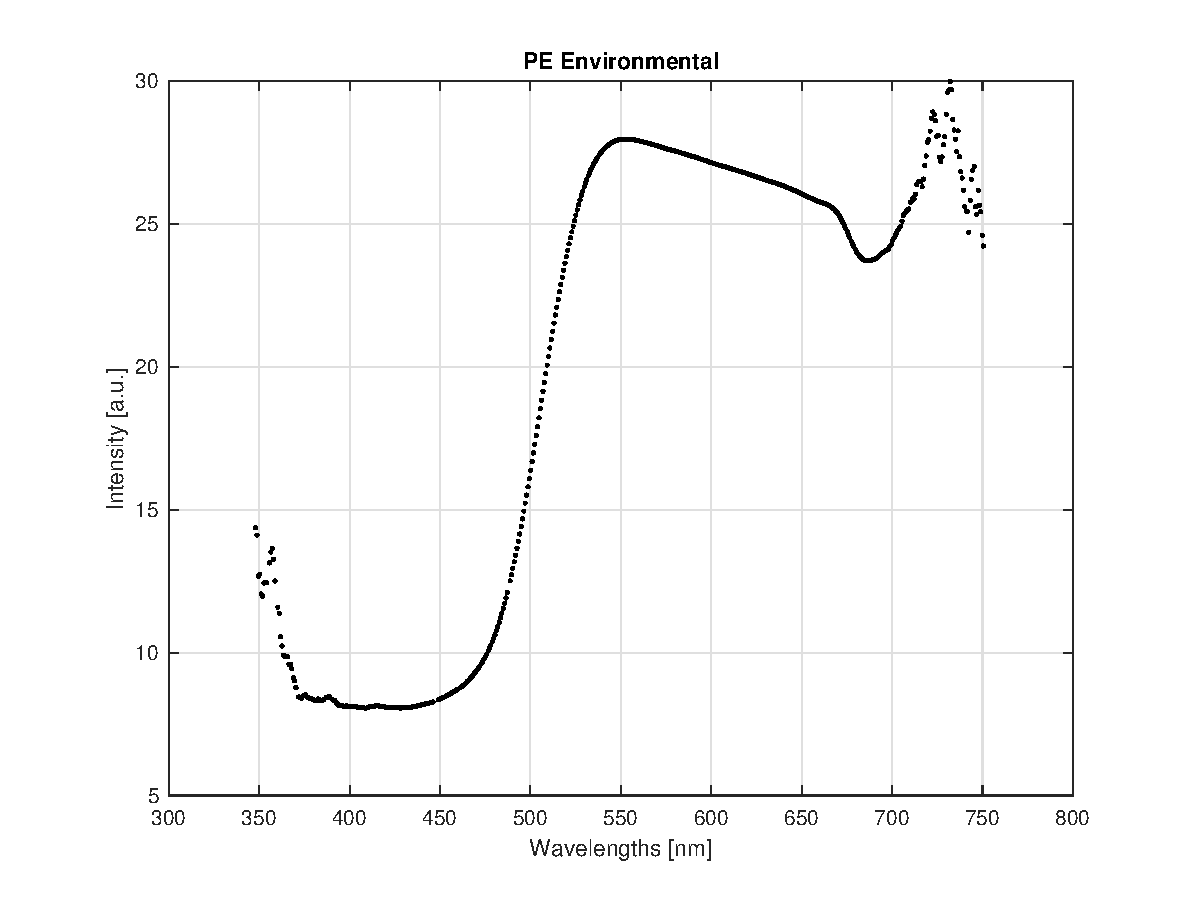
\includegraphics[scale=0.36]{Images/appendix/p-env_yellowbowl.eps}}
  \begin{minipage}{\wd\FigBox}
    \centering\usebox{\FigBox}
    \subcaption{a) PE Environment}
  \end{minipage}
    % Top image is centered, so no need to get width
 \sbox{\FigBox}{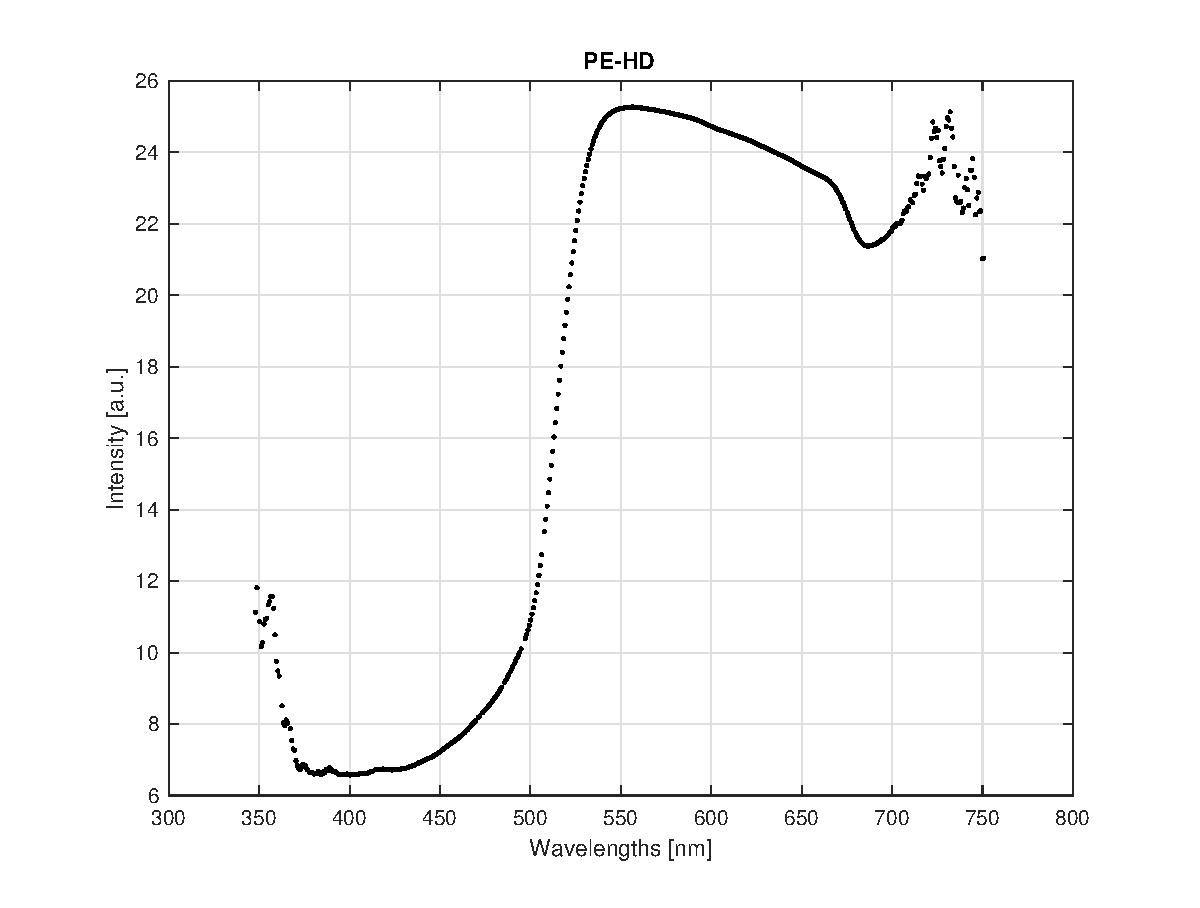
\includegraphics[scale=0.36]{Images/appendix/pe-hd-postconsum.eps}}
  \begin{minipage}{\wd\FigBox}
    \centering\usebox{\FigBox}
    \subcaption{b) PE-HD Post Consumer}
  \end{minipage}
  % Save second image 
  \caption{A comparison of the resulting signature for  and PVC - both in a yellow color}
  \label{fig:plastcomp1}
\end{figure}
\end{comment}


\noindent
As can be seen from Figure \ref{fig:plastcomp1}, the signatures of the two types are almost identical, with a possibility of deviations due to measurements errors. From Section \ref{sec:microplastic}, we know for a fact that the structure of these two are very different. PP contains several molecules with the chemical formula of $C_3H_6$, while PVC has molecules with the following formula, $C_2H_3Cl$, even containing additional chlorine-atoms, Cl.  
\\\\
\subsection{Various Colors}
Another result is from the more colorful pieces of microplastics. Figures \ref{fig:green}, \ref{fig:red} and \ref{fig:blue} display the resulting signatures of green-colored PE-HD, red-colored PE-HD and blue-colored PE-LD, with their associated wavelength circled on the visible light spectrum.  
%grønn
\begin{figure}[H]
  \newcommand*\FigVSkip{0.5em}
  \newcommand*\FigHSkip{0.1em}
  \newsavebox\FigBox
  \centering
% Top image is centered, so no need to get width
 \sbox{\FigBox}{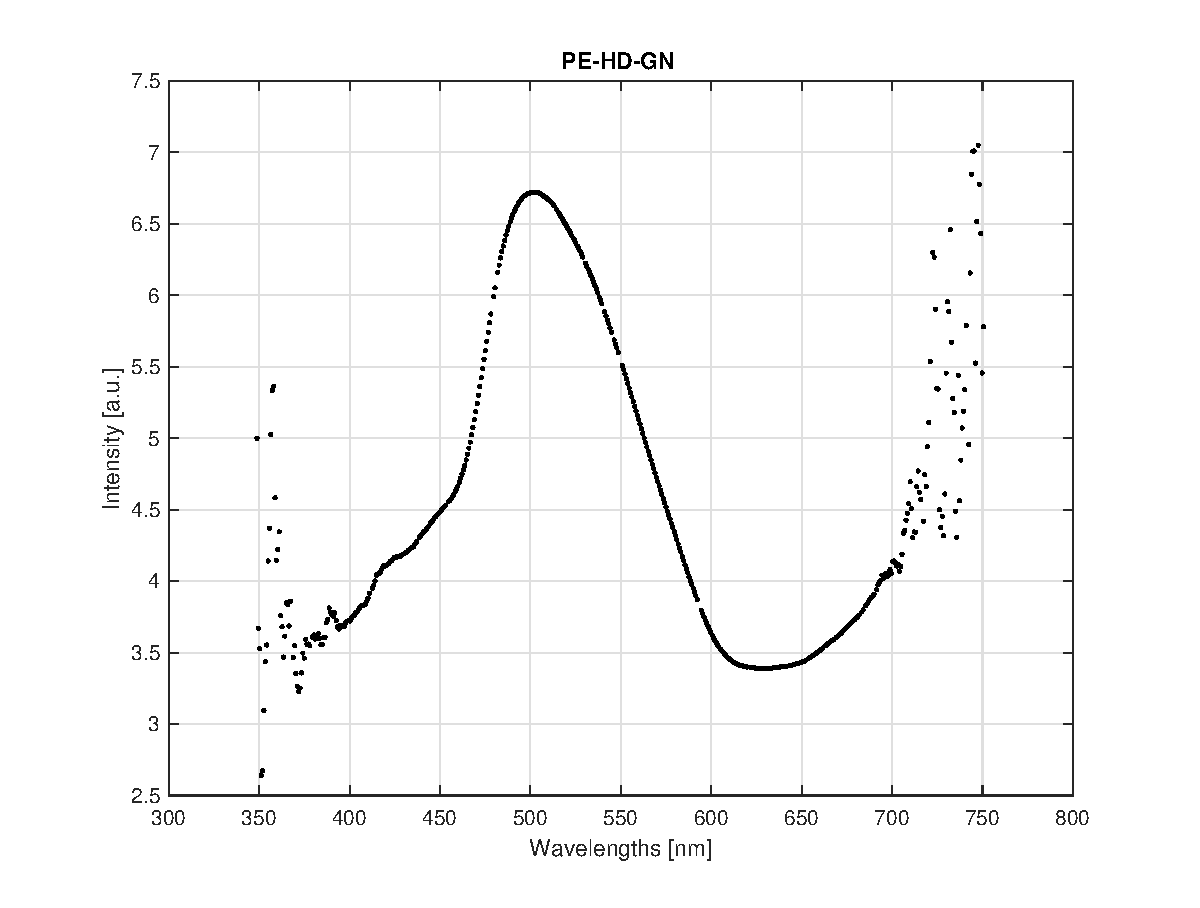
\includegraphics[scale=0.36]{Images/appendix/pe-hd-postconsumer-green.eps}}
  \begin{minipage}{\wd\FigBox}
    \centering\usebox{\FigBox}
    \subcaption{a) PE-HD Post Consumer, Green}
  \end{minipage}
  % Save second image 
  % Top image is centered, so no need to get width
 \sbox{\FigBox}{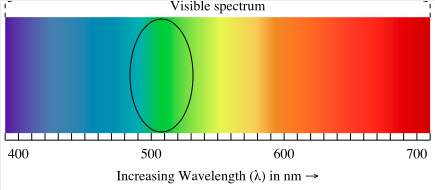
\includegraphics[scale=0.4]{Images/results/specgreen.png}}
  \begin{minipage}{\wd\FigBox}
    \centering\usebox{\FigBox}
    \subcaption{b) The visible light spectrum, circled at green}
  \end{minipage}
  \caption{A comparison of the resulting signature for green-colored PE-HD and the visible light spectrum-reference}
  \label{fig:green}
\end{figure}

%red
\begin{figure}[H]
  \newcommand*\FigVSkip{0.5em}
  \newcommand*\FigHSkip{0.1em}
  \newsavebox\FigBox
  \centering
  % Top image is centered, so no need to get width
 \sbox{\FigBox}{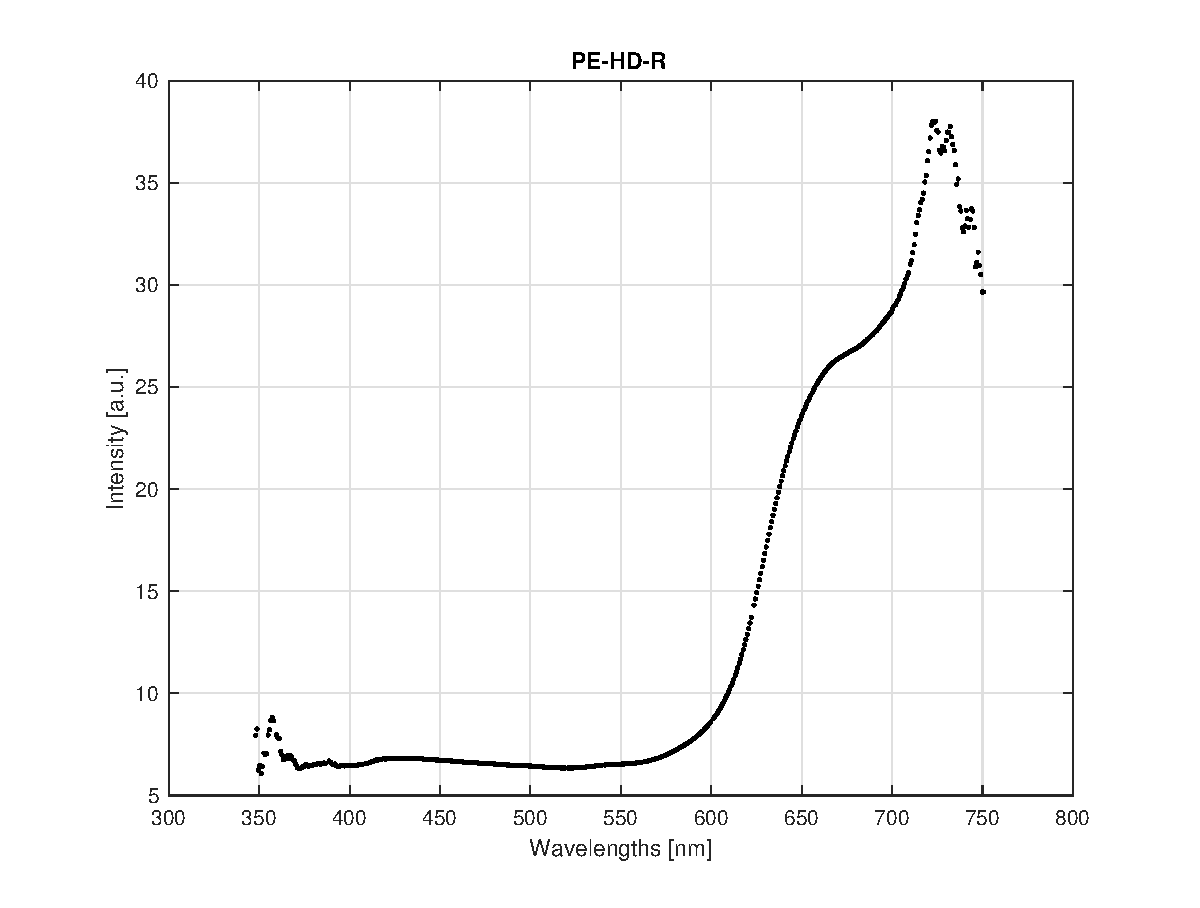
\includegraphics[scale=0.36]{Images/appendix/pe-hd-postconsum-red.eps}}
  \begin{minipage}{\wd\FigBox}
    \centering\usebox{\FigBox}
    \subcaption{a) PE-HD Post Consumer, Red}
  \end{minipage}
    % Top image is centered, so no need to get width
 \sbox{\FigBox}{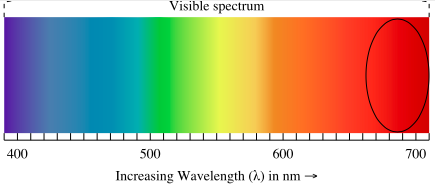
\includegraphics[scale=0.4]{Images/results/specred.png}}
  \begin{minipage}{\wd\FigBox}
    \centering\usebox{\FigBox}
    \subcaption{b) The visible light spectrum, circled at red}
  \end{minipage}
  % Save second image 
  \caption{A comparison of the resulting signature for red-colored PE-HD and the visible light spectrum-reference}
  \label{fig:red}
\end{figure}

%blue
\begin{figure}[H]
  \newcommand*\FigVSkip{0.5em}
  \newcommand*\FigHSkip{0.1em}
  \newsavebox\FigBox
  \centering
  % Top image is centered, so no need to get width
 \sbox{\FigBox}{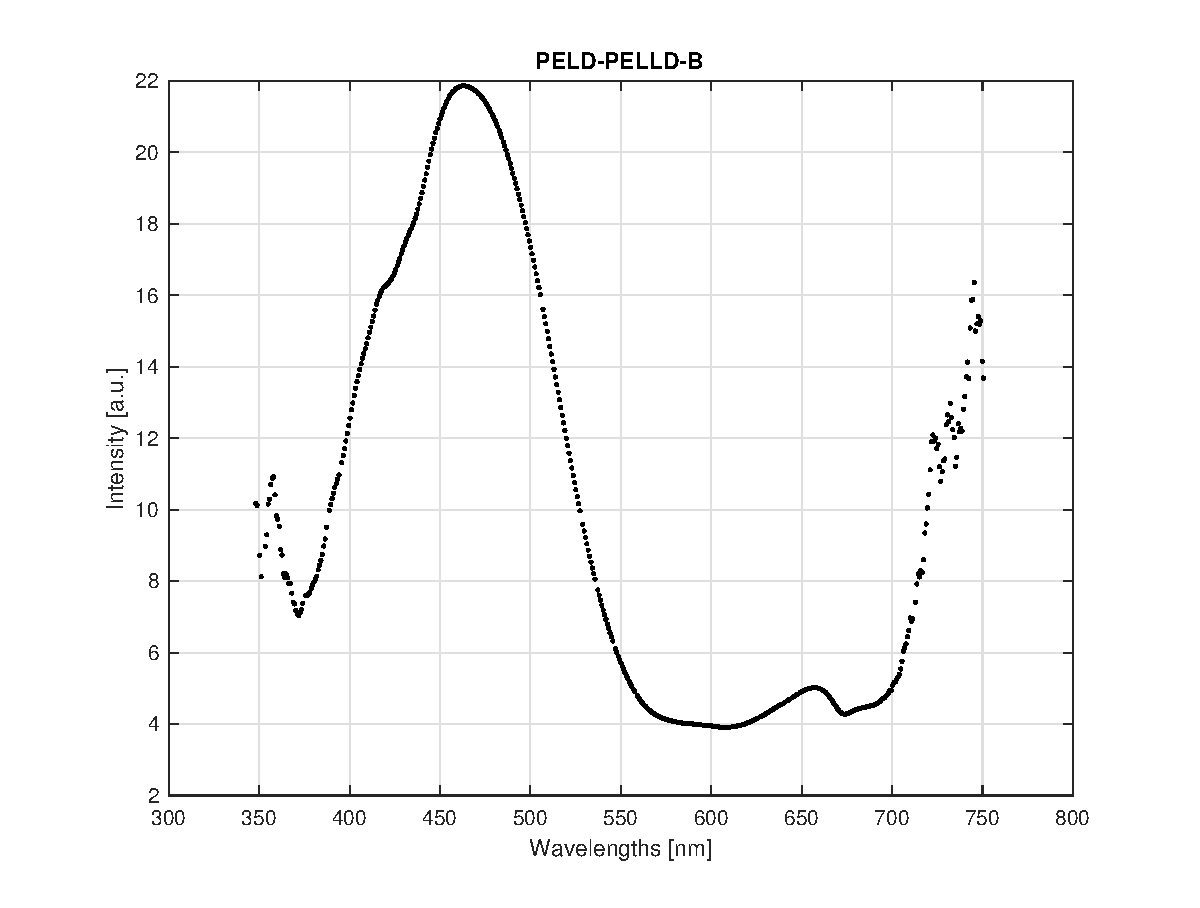
\includegraphics[scale=0.36]{Images/appendix/pe-ld-postindust-blue.eps}}
  \begin{minipage}{\wd\FigBox}
    \centering\usebox{\FigBox}
    \subcaption{a) PE-LD Post Industrial, Blue}
  \end{minipage}
    % Top image is centered, so no need to get width
 \sbox{\FigBox}{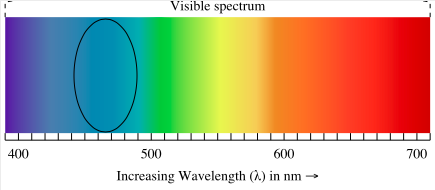
\includegraphics[scale=0.4]{Images/results/specblue.png}}
  \begin{minipage}{\wd\FigBox}
    \centering\usebox{\FigBox}
    \subcaption{b) The visible light spectrum, circled at blue}
  \end{minipage}
  % Save second image 
  \caption{A comparison of the resulting signature for blue-colored PE-LD and the visible light spectrum-reference}
  \label{fig:blue}
\end{figure}

%kilde for visible light reference
%https://www.khanacademy.org/science/physics/light-waves/introduction-to-light-waves/a/light-and-the-electromagnetic-spectrum

\noindent
This result support the earlier assertion about the color being dominant when detecting the spectral image of the plastic. Figures \ref{fig:green} and \ref{fig:red} are even the result of the same type of plastic, PE-HD. However, there is not much resemblance in the plots.
\\\\
The color variation is also found from the PCA as the second principal component. It is therefore reasonable to conclude that the specific color has a large influence.
\\\\
\subsection{Various Sizes}
Another interesting comparison is the result of the same type of plastic, in different sizes. In this section, illustrated by Figure \ref{fig:size}, a clear empty bottle of Farris, existent of PET-plastic, is compared to clear PET Amorphous. The pieces of PET Amorphous are 3mm thick, while the piece from the bottle is significantly larger. 

\begin{figure}[H]
  \newcommand*\FigVSkip{0.5em}
  \newcommand*\FigHSkip{0.1em}
  \newsavebox\FigBox
  \centering
  % Top image is centered, so no need to get width
 \sbox{\FigBox}{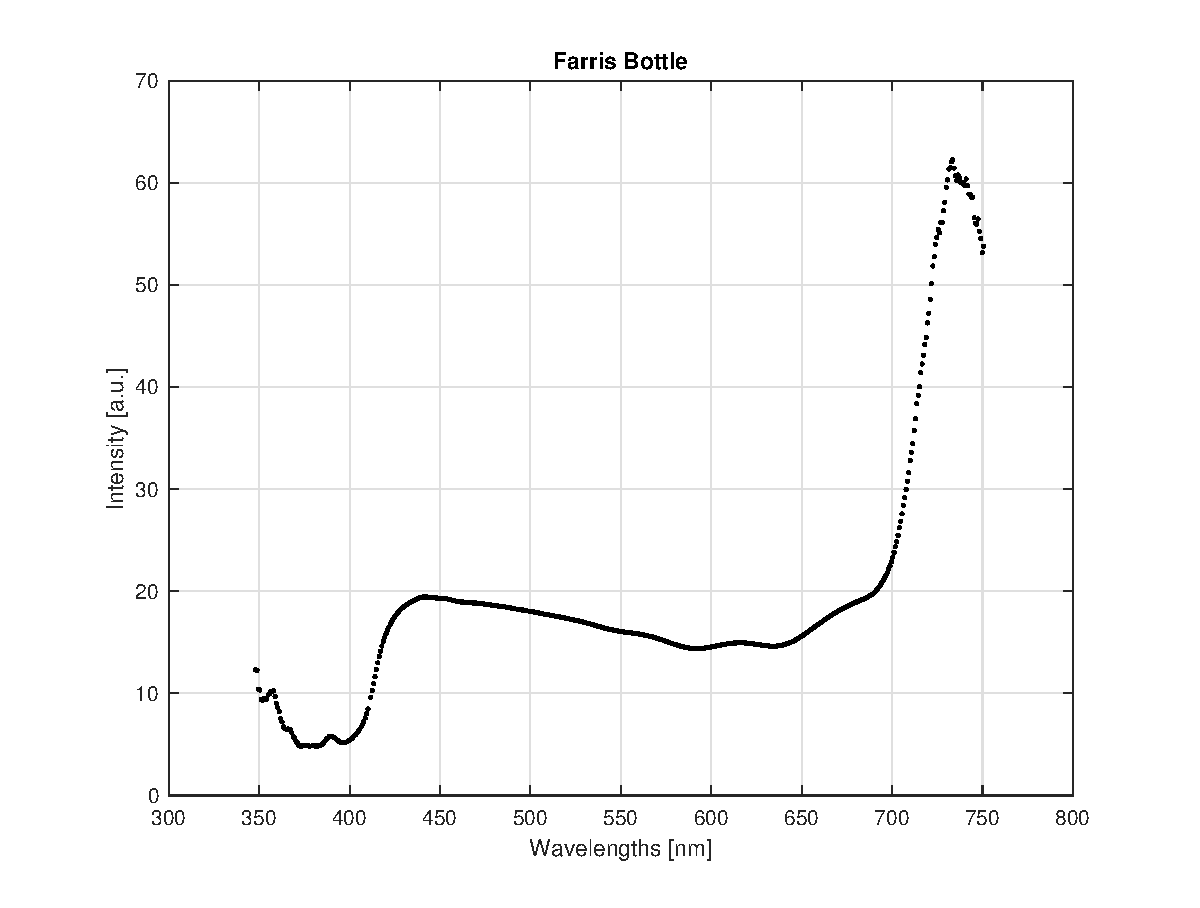
\includegraphics[scale=0.36]{Images/appendix/farris.eps}}
  \begin{minipage}{\wd\FigBox}
    \centering\usebox{\FigBox}
    \subcaption{a) Clear Farris Bottle}
  \end{minipage}
    % Top image is centered, so no need to get width
 \sbox{\FigBox}{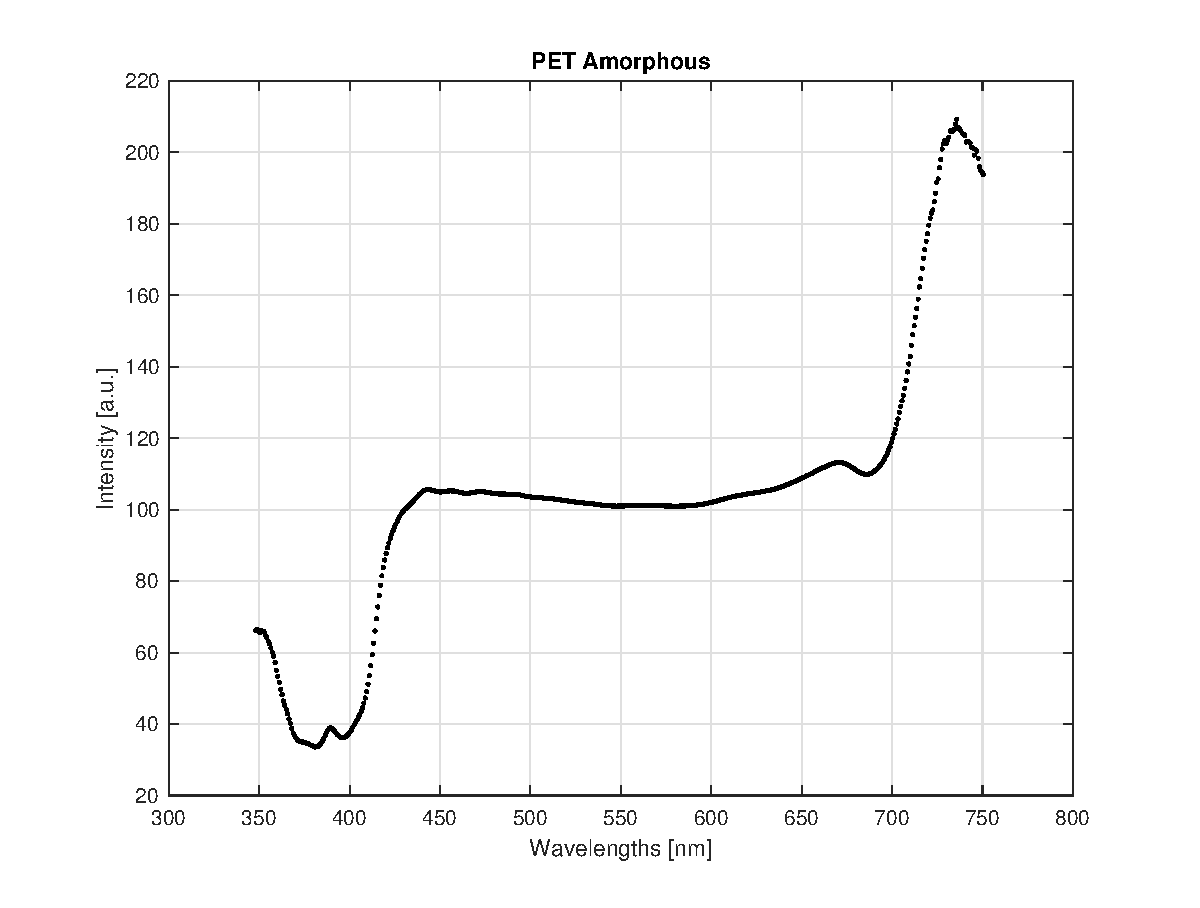
\includegraphics[scale=0.36]{Images/appendix/pet-amorphous-pristine-clear.eps}}
  \begin{minipage}{\wd\FigBox}
    \centering\usebox{\FigBox}
    \subcaption{b) Clear PET Amorphous}
  \end{minipage}
  % Save second image 
  \caption{A comparison of a large PET piece from a Farris bottle and tiny PET Amorphous pieces}
  \label{fig:size}
\end{figure}
\noindent
When comparing the resulting signatures above, it is clear that they share trends. A quick look at Figure \ref{fig:size} reveals many similarities. Nevertheless, looking at the y-axis displaying intensity, one can observe a tripled intensity from the microplastic. 





\section{Discussion}
\label{sec:discussion}
 In this chapter several aspects of the project thesis will be discussed.
 
 %Klassifisering basert på PCA-resultatene
 

 
 
 
\section{Signatures Directly Interpreted}
In order to obtain a color-free spectrum, one could subtract the color spectrum from the resulting spectrum retrieved from the experiments. However, most pieces of plastic do not have one specific color, making it difficult to determine the spectrum to subtract. 
\\\\
In addition, when experimenting with different types of plastics having more or less the same colors, the results turned out next to identical. At first, a thought was that this was due to the color being too dominant in relation to the rest of the properties. However, conducting the same experiment with non-colored pieces of plastic, gave the same end-result; no difference in spectral signature even if the types of plastics differ. - could this be due to reflectance disturbance from "shiny" see through material, or is it in fact impossible to distinguish the different types from each other using hyperspectral imaging in visible light?
\\\\
Discussing the size-difference. Also, why is the intensity this different?
 
\section{Sources of Error}
Due to the ambient environment and sensors related to Hyper Spectral Imaging noise will be next to impossible to exclude. There is always some dark noise due to the sensors of the system. Also, since the measured values are based of a ratio rather than absolute values small changes could have large outcomes due to the fact that the values are divided by extremely small values. A change in the divisor may be small, but the outcome large due to the relative change. However, the tests were limited to the visible spectrum, whereas the biggest variation were in the infrared or near-infrared spectrum. Even though there were variations in the visible spectrum the results were satisfactory with respect to change due to noise. 
\\\\
Furthermore, the ambient light in the room is hard to completely avoid. Even though all light was turned off and blinds were used some light still got in. The light will affect the results, and could possibly affect the signature. However, due to the low amount of lighting that were present during the tests, it is assumed that it did not have a considerable effect on the results. The ambient light is therefore assumed to be negligible. 
\\\\
Even though the plastic was order specially in order to have pure samples, there are still sources that are unknown. As a result, the results could be affected by the differences in the plastic composition made by the manufacturer. However, the results showed a clear tendency where the actual color of the plastic was dominant as opposed to the chemical composition.
\\\\
The see-through plastic will be affected by the background. Compensating for the paper was not performed, and the results were most likely is affected by the background. The effect is not completely clear, but the trend of see through plastic have a similar peak to paper is could display the effect of the background. On the other hand, the background would most likely affect the results of the clear plastic either way. Therefore, the results were deemed satisfactory with the white background.
\\\\
The scanning was easily affected by the movement of the scanner. This was portrayed in the change of the reflectance standard. It is therefore a concern that the same effect will have caused the signatures to be inconsistent. However, the reflectance was regularly updated and there was several measurements per plastic type in order to account for large individual variations. It is still a concern that single measurements that were affected could skew the results.
\\\\


\section{Nothing but thoughts for now..}
VISUAL LIGHT:
Experiments analyzing the wave spectra of different types of plastics, have already been conducted. However, the results have been directed towards viewing the wave length interval describing near infrared light (NIR). Although the use of infrared light is an effective means of unobtrusive observation on land, it is far less effective in the ocean because long wavelength light is rapidly attenuated by seawater. One can therefore discuss whether it is possible to detect microplastic underwater with NIR. Is it possible to get close enough? etc..
\\\\
%https://oceanoptics.com/plastic-recycling-nir-spectroscopy/
Another important observation in these experiments, is the condition of the microplastic used. The material is pure and white, making the results independent of color. 
\\\\
%Water absorption 
%https://commons.wikimedia.org/wiki/File:Absorption_spectrum_of_liquid_water.png
%This logarithmic (log-log) graph shows water’s absorption behavior at different colors wavelength. As seen in the graph, water absorption is minimized between 400 -600 nm


%Light Transmission in the Ocean: http://www.waterencyclopedia.com/La-Mi/Light-Transmission-in-the-Ocean.html
%https://manoa.hawaii.edu/exploringourfluidearth/physical/ocean-depths/light-ocean

\\\\
\noindent
AN IDEA: 
What if we could inspect the level of additive acceptance in the different types of plastic. By finding the most resistant types, it might be possible to modify these into doing the same job as the types accepting additives. This way, we could reduce the production of the largest vectors/toxin-carriers. 

\todo[inline, color = red!60]{geir snakker om florescence of ditto lyssetting}